\documentclass[11pt]{report}
\usepackage[utf8]{inputenc}
\usepackage{comment,times}
\usepackage{xurl}
\usepackage{hyperref}
\usepackage{graphicx}
\usepackage[table,xcdraw]{xcolor}
\usepackage[caption=false]{subfig}
\usepackage{caption}
\usepackage{enumitem}
\usepackage{longtable}
\usepackage{setspace}
\usepackage[skip=20pt plus1pt, indent=20pt]{parskip}
\usepackage{atbegshi}

\usepackage{algorithm}
\usepackage[noend]{algpseudocode}
\newcommand{\vars}{\texttt}
\newcommand{\func}{\textrm}
\let\oldReturn\Return
\renewcommand{\Return}{\State\oldReturn}
\newcommand*\Let[2]{\State #1 $\gets$ #2}
\algrenewcommand\alglinenumber[1]{
  {\sf\footnotesize\addfontfeatures{Colour=888888,Numbers=Monospaced}#1}
}
\algrenewcommand\algorithmicrequire{\textbf{Precondition:}}
\algrenewcommand\algorithmicensure{\textbf{Postcondition:}}


\textwidth 6.5in
\textheight 9.5in
\oddsidemargin 0pt
\evensidemargin 0pt
\topmargin -67pt

\captionsetup{font=footnotesize}
% \AtBeginDocument{\AtBeginShipoutNext{\AtBeginShipoutDiscard}}
% \renewcommand{\chaptername}{Section}
\newcommand{\monolithicPR}{Algorithm \textsc{DynamicMonolithicPR}}
\newcommand{\levelwisePR}{Algorithm \textsc{DynamicLevelwisePR}}
\newcommand{\X}{$\times$}
\newcommand{\x}{$\times$}




\title{
  Exploring Optimizations for Dynamic Graph Algorithms on the GPU \\
  {\small Comprehensive Report}
  {
\includegraphics[width=0.99\textwidth]{out/logo-iiit.jpg}}
}
\author{
  \textbf{Subhajit Sahu} \\
  \textbf{Advisor: Kishore Kothapalli} \\
  Center for Security, Theory, and Algorithmic Research (CSTAR) \\
  International Institute of Information Technology, Hyderabad (IIITH) \\
  Gachibowli, Hyderabad, India - 500 032 \\
  subhajit.sahu@research.iiit.ac.in
}




\begin{document}
\maketitle
\tableofcontents
%\onehalfspacing

\chapter{Introduction}
The Königsberg bridge problem, which was posed and answered in the negative by Euler in 1736 represents the beginning of graph theory \cite{graph-weisstein}. A \textbf{graph} is a generic data structure and is a super set of lists, and trees. Social networks, co-author networks, citation networks, computer networks, road networks, (artificial) neural networks, and financial networks are are real-life manifestations of graphs. \textbf{Interaction} between messenger molecules in the body, interaction between people on social media, and spreading of infectious diseases, are also modelled as graphs. Finding the shortest \textbf{path} between two points, and \textbf{sorting web pages} in order of importance are also graph problems. Graphs are indeed unifying abstractions that can leverage interconnectedness to represent, predict, and explain several phenomena \cite{graph-sakr21}.
% The \textbf{assignment of registers} to variables (by compiler), and the assignment of \textbf{available channels} to a radio transmitter are also graph problems. 

\textbf{Static graphs} are those which do not change with time. Static graph algorithms are techniques used to solve such a graph problem (developed since the 1940s). Static algorithms are also known as off-line or start-over algorithms \cite{incr-ramalingam96}. To solve problems on larger and larger graphs, a number of optimizations (both algorithmic and hardware/software techniques) have been developed to take advantage of \textbf{vector-processors} (like Cray), \textbf{multicores}, and \textbf{GPUs}. A lot of research had to be done in order to find ways to enhance parallelism. The techniques include a number of \textbf{parallel algorithms}, \textbf{concurrency models}, \textbf{locking techniques}, \textbf{transactions}, etc. This is especially due to a lack of \emph{single-core performance} improvements.

Graphs where relations vary with time, are called \textbf{dynamic graphs}. The updates to these relations can be changes, insertions, or deletions of vertices / edges. Many problems use dynamic graphs. These dynamic graphs can be thought of as a series of static graphs at different points in time. In order to solve graph problems on these dynamic graphs, one possibility is to take the graph at a certain point in time, and run the necessary static graph algorithm on it. However, as the size of the dynamic graph grows, this repeated computation becomes increasingly slower. It is possible to take advantage of previous results, in order to compute the result for the next time point. Such algorithms are called \textbf{dynamic graph algorithms}, or on-line graph algorithms \cite{incr-ramalingam96}.

Interactive systems such as program development, document writing, and computer-aided design (CAD) where the users build and update an object gradually, and the object has to repeatedly processed in some fashion as it is being built up cannot be supported with static algorithms \cite{incr-ramalingam96}. Since the inception of the Internet and the World Wide Web (WWW), the web graph has been growing at an exponential rate. Given that this web graph is being constantly updated, search engines must repeatedly update their rankings of web pages in order to generate relevant (recent) search results. However, the sheer size of the web graph they need to process makes using a static algorithm unacceptable. Applications such as these make the study of parallel dynamic graph algorithms relevant.

A static algorithm $f(\cdot)$ is one which takes in an input graph $x$ and generates an output $y$, as shown in Figure \ref{fig:about-static-vs-dynamic-algorithm}. On the other hand, a dynamic algorithm $g(\cdot)$ accepts the original input $x$, the original output $y$, and importantly the change in input $\Delta x$, and provides us with the updated output $y + \Delta y$ as shown in Figure \ref{fig:about-static-vs-dynamic-algorithm}. It may also accept an additional auxiliary information as input, and generate an output auxiliary information. The objective is to identify the part of the output which is no longer correct, and update it. If it is not possible to exactly determine the part of the affected output, and hence the part of the input that needs to be processed, we should overestimate it \cite{incr-ramalingam96}.

The efficiency of a dynamic algorithm depends on how well that affected part if the output is estimated from the change in input. As long as the change in output is sufficiently small, the actual size of the input should in general not affect the execution required by the algorithm. The efficiency of dynamic algorithms also depends upon the overhead for determining the part of input that needs to be processed. Unlike a static graph algorithm, where the worst-case time complexity (using big-$O$ notation) is expressed in terms of input size parameters, such as $n$ (total number of vertices in the graph) and $m$ (total number of edges in the graph); the time complexity of a dynamic algorithm is expressed in terms of change in input and the associated affected output $\delta$ size, which is usually written as $||\delta||$. It should be noted that there exist unbounded dynamic graph problems, where the worst-case time complexity has to be expressed in terms of the size of original input. Dynamic algorithms for such problems may still perform better than static algorithms, in the average case \cite{incr-ramalingam96}.

\begin{figure}[hbtp]
  \centering  % \vspace{-0.3 cm}
  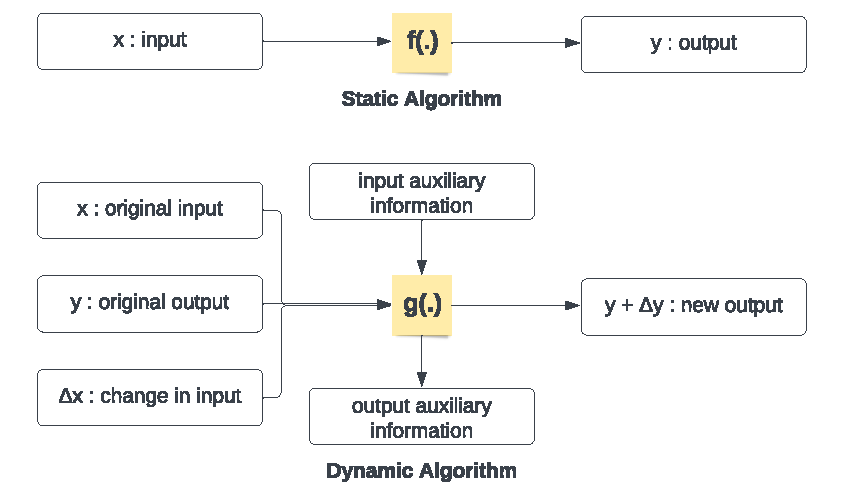
\includegraphics[width=0.70\textwidth]{out/about-static-vs-dynamic-algorithm.pdf}
  \caption{Comparison of a \emph{static} and a \emph{dynamic} algorithm. \cite{incr-ramalingam96}.}
  \label{fig:about-static-vs-dynamic-algorithm}
\end{figure}



A dynamic algorithm can be incremental, decremental, or fully dynamic. Incremental algorithms are those which only consider additions to the initial graph (possibly starting from empty graph), while decremental algorithms only consider only deletions to the initial graph (such as decremental Breadth-First Search or BFS by Shiloach et al. \cite{bfs-shiloach81}). Incremental and decremental algorithms are also collectively known as partially dynamic algorithms. \textbf{Fully dynamic algorithms}, on the other hand, consider both additions and deletions to the graph \cite{graph-italiano99} (such as fully dynamic Transitive closure by King et al. \cite{closure-king08}).

A fully dynamic graph algorithm can accept one or more vertex/edge insertions/deletions. When it accepts a \textbf{batch} (multiple) of insertions and deletions, it is known as a batched fully dynamic graph algorithm. Processing multiple changes to the graph allows the algorithm to amortize the cost of requisite computation on the affected region of the graph, as well as the overhead associated with determining this affected region. The appropriate choice of batch size depends upon frequency and size of updates to the input, and the required frequency of output updates.

The study of parallel dynamic graph algorithms is an ongoing area of research, which includes new algorithms, hardware/software optimization techniques for distributed systems, multicores (shared memory), GPUs, and even FPGAs. Optimization of algorithms can focus on \textbf{space complexity} (memory usage), \textbf{time complexity} (query time), \textbf{preprocessing time}, and even \textbf{accuracy of result}.

% While dynamic algorithms only focus on optimizing the algorithm’s computation time, \textbf{dynamic graph data structures} focus on improving graph update time, and memory usage. Dense graphs are usually represented by an adjacency matrix (bit matrix). Sparse graphs can be represented with variations of adjacency lists (like CSR), and edge lists. Sparse graphs can also be thought of as sparse matrices, and edges of a vertex can be considered a bitset. In fact, a number of graph algorithms can be modeled as \textbf{linear algebra} operations (see \textbf{nvGraph} \footnote{https://github.com/rapidsai/nvgraph}, \textbf{cuGraph} \footnote{https://github.com/rapidsai/cugraph} frameworks). A number of dynamic graph data structures have also been developed to \textbf{improve update speed} (like Packed-Memory Array or PMA), or \textbf{enable concurrent updates} and computation (like \textbf{Aspen's} \footnote{https://github.com/ldhulipala/aspen} compressed functional trees) \cite{graph-besta19}. These data formats are illustrated in Figure \ref{fig:about-graph-representation}.

% \begin{figure*}[hbtp]
  \centering
  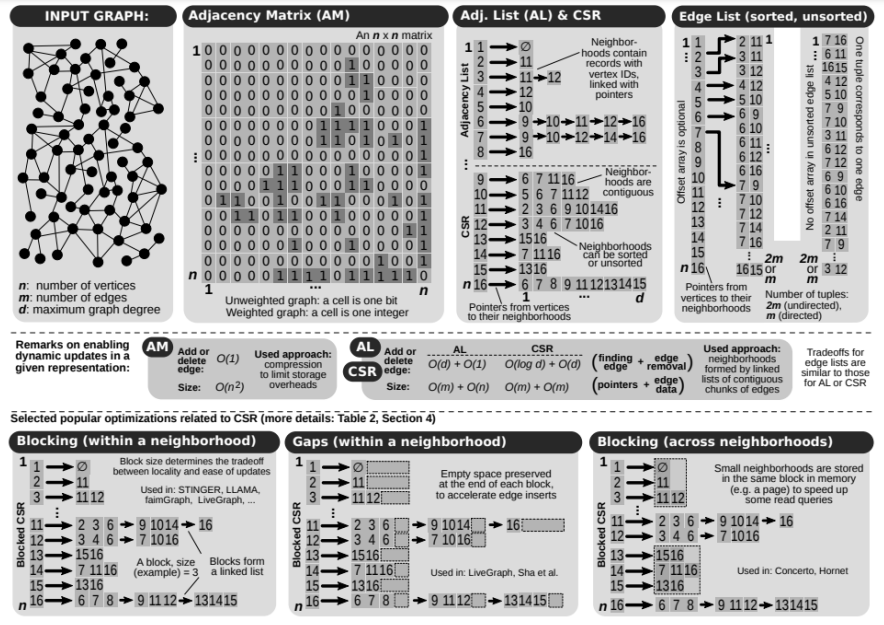
\includegraphics[width=0.98\textwidth]{out/about-graph-representation.png}
  \caption{Illustration of fundamental graph representations (Adjacency Matrix, Adjacency List, Edge List, CSR) \cite{graph-besta19}.}
  \label{fig:about-graph-representation}
\end{figure*}



Streaming / dynamic / time-evolving \textbf{graph data structures} maintain only the latest graph information \cite{graph-besta19}. Streaming graphs can grow indefinitely as new data arrives. They are typically unbounded, thus the underlying systems are unable to keep the entire graph state \cite{graph-sakr21}. \textbf{Historical graphs} on the other hand keep track of all previous states of the graph. Changes to the graphs can be thought of as \textbf{edge insertions}, \textbf{deletions}, or \textbf{updates}, which are sometimes done in batches. Insertions and deletions on streaming graphs are considered as arrivals and removals from a sliding window \cite{graph-sakr21}. Except for functional techniques, updating a graph usually involves modifying a \textbf{shared structure} using some kind of fine-grained synchronization. It might also be possible to store additional information along with vertices/edges, though this is usually not the focus of research (graph databases allow storage of associated data and labels).

In conclusion, we are in the midst of an unprecedented growth of interconnected data, and graph processing systems are expected to play a vital role. These systems rely on complex runtimes that combine software and hardware platforms, which make fair performance measurement and benchmarking difficult. There is a lack of a widely used performance metric other than response time \cite{graph-sakr21}. We intend to focus on the \textbf{design and implementation of dynamic and streaming graph algorithms in the parallel and the distributed setting}, while following suitable approaches for measuring performance and comparing across alternative methods.




% Figure \ref{fig:about-graph-processing} illustrates a complex pipeline for graph processing.
% \begin{figure}[hbtp]
  \centering
  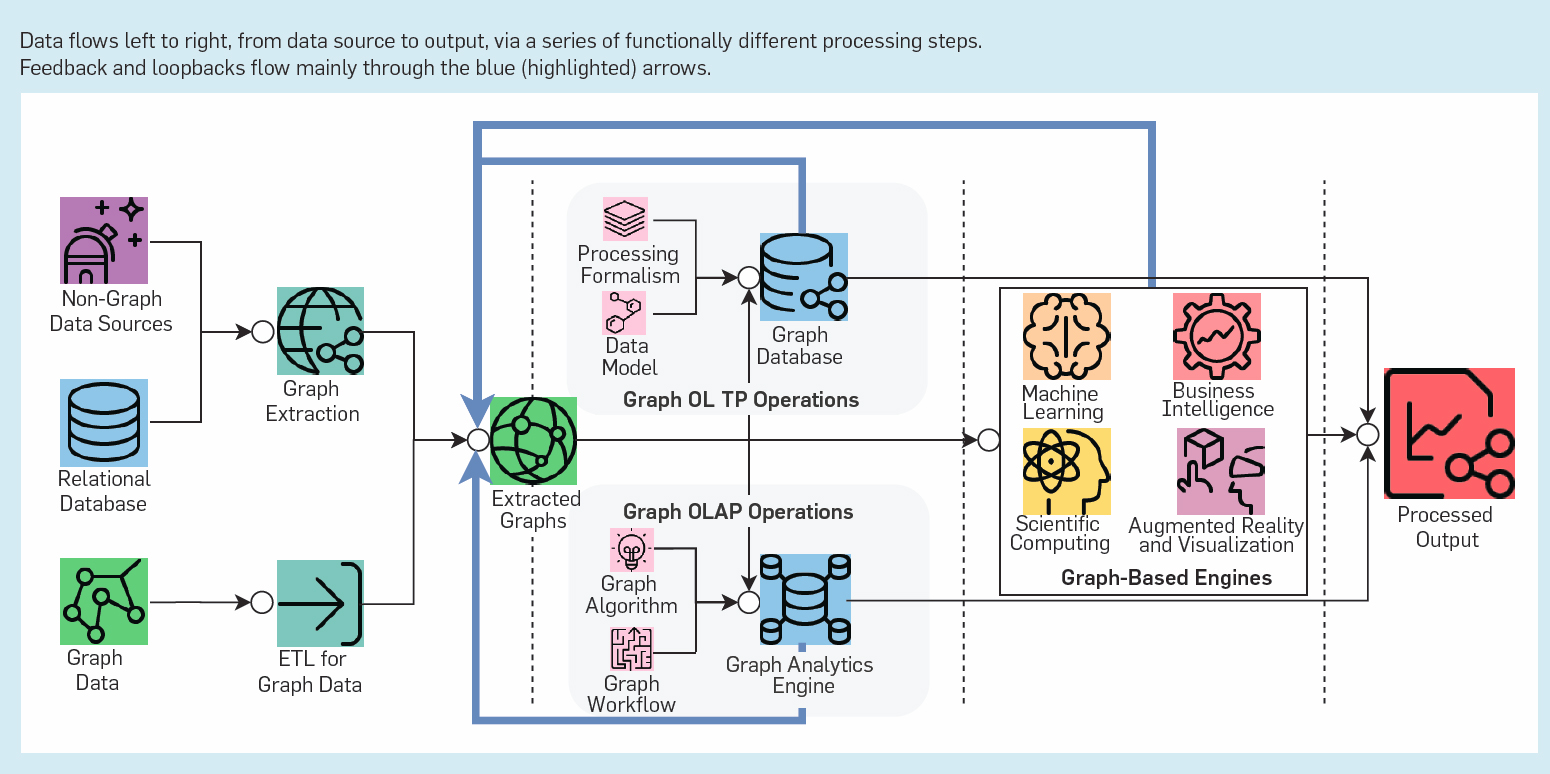
\includegraphics[width=0.98\textwidth]{out/about-graph-processing.jpg}
  \caption{Illustration of a complex data pipeline for graph processing \cite{graph-sakr21}.}
  \label{fig:about-graph-processing}
\end{figure}


% In the recent decade or so, a number of \textbf{graph streaming frameworks} have been developed, each with a certain focus area, and targeting a certain platform (distributed system / multiprocessor / GPU / FPGA / ASIC). Such frameworks focus on designing an improved dynamic graph data structure, and define a fundamental model of computation. For \textbf{GPUs}, the following frameworks exist: \textbf{cuSTINGER}, \textbf{aimGraph}, \textbf{faimGraph} \footnote{https://github.com/GPUPeople/faimGraph}, \textbf{Hornet} \footnote{https://github.com/hornet-gt/hornet}, \textbf{EvoGraph} \footnote{https://github.com/chan150/EvoGraph}, and \textbf{GPMA} \footnote{https://github.com/desert0616/gpma\_demo} \cite{graph-besta19}.
% In conclusion, we are in the midst of an unprecedented growth of interconnected data, and graph processing systems are expected to play a vital role. Figure \ref{fig:about-graph-processing} illustrates a complex pipeline for graph processing. However, the following challenges come up in the design of big graph processing systems \cite{graph-sakr21}:
% \begin{itemize}[itemsep=-1.5em,topsep=0em]
% \item These systems rely on complex runtimes that combine software and hardware platforms, which make fair performance measurement and benchmarking difficult. There is a lack of a widely used performance metric other than response time.
% \item There is considerable tension between performance-oriented specialized graph processing stacks, and productivity-oriented ones that support portability and interoperability. More than 100 big graph processing systems exist, but they do not support portability.
% \item Comprehensive large-scale graph processing experiments lack tractability due to the inability to implement, deploy, and experiment within a reasonable amount of time and cost.
% \item Users have to choose from a large spectrum of graph data models that are similar but differ in terms of expressiveness, cost, and intended use for querying and analytics.
% \item No standard graph library or query language currently exists. However, the Graph Query Language (GQL) standardization project is in progress.
% \end{itemize}


\chapter{Literature survey}
Dynamic graph algorithms support query operations of certain properties on a dynamic graph \cite{graph-italiano99}. Examples of such algorithms include \emph{Dynamic Connectivity (undirected graph)} which tells whether the graph is connected or two given vertices are connected through edges \cite{conn-patrascu04}, \emph{Dynamic Transitive Closure (directed graph)} which tells whether a vertex is reachable from another vertex \cite{conn-demetrescu00}, \emph{Dynamic All Pairs Shortest Path (APSP)} which tells the shortest path and distance between any two vertices \cite{apsp-demetrescu04}, \emph{Dynamic Minimum Spanning Tree (MST)} which determines the value of a property on an MST \cite{mst-henzinger97}, \emph{Dynamic Min Cut} which tells whether two vertices are on the same side on a minimum cut \cite{cut-italiano11}, \emph{Dynamic Planarity} which tells whether the graph is planar (the edges do not cross each other) \cite{planar-galil99}, or \emph{Dynamic k-connectivity} which tells whether the graph is k-connected or whether two given vertices are k-connected (removing fewer than k vertices still maintains connectivity) \cite{conn-liang01} \cite{graph-italiano99}.

Dynamic Centrality, which was first developed in social network analysis \cite{graph-newman18}, is an important category of dynamic graph algorithms which focus on ranking vertices in a graph based on an importance metric \cite{centrality-bonacich87}. It finds applications in identifying super-spreaders of a disease, key infrastructure nodes in the Internet or mobile networks, the most informative websites, influential person(s) in a social network \cite{centrality-borgatti05}, and brain networks \cite{brain-vandenheuvel13} \cite{brain-saberi21}. Importance is conceived as a type of flow across the network, or an involvement in cohesiveness of the network. Eigenvector centrality which measures the influence of a vertex in a graph is a walk based importance metric, and is based on the concept that contributions from important vertices are more important \cite{graph-newman16}. PageRank centrality is a variation of Eigenvector centrality, which measures the importance of a vertex based on its in-bound edges instead of out-bound ones and includes a scaling factor per graph \cite{pr-network20q}.

% Dynamic Centrality, which was first developed in social network analysis \cite{graph-newman18}, is an important category of dynamic graph algorithms which focus on ranking vertices in a graph based on an importance metric \cite{centrality-bonacich87}. It finds applications in identifying super-spreaders of a disease, key infrastructure nodes in the Internet or mobile networks, the most informative websites, influential person(s) in a social network \cite{centrality-borgatti05}, and brain networks \cite{brain-vandenheuvel13} \cite{brain-saberi21}. Importance is conceived as a type of flow across the network, or an involvement in cohesiveness of the network. For a flow-based importance metric, the flow can be conserved (like package delivery) or duplicate-able (like gossip spread); the paths can constrained to geodesics (shortest paths), paths (visit vertices once), trails (visit edges once) or walks (no limit); walks can be made from a given vertices (radial), or through a given vertex (medial); and the counting can capture walk volume (total number of walks), or walk length (distance from given vertex to remaining vertices) \cite{centrality-borgatti05} \cite{centrality-borgatti06}.

% A centrality which is optimal for one application is often sub-optimal for another application, and is the reason why we need so many different centralities \cite{politics-krackhardt90}. It should also be noted that centrality algorithms focus obtaining the most important vertices, and the rankings do not necessarily generalize to the remaining vertices \cite{centrality-lawyer15} \cite{epidemic-dasilva12} \cite{epidemic-bauer12} \cite{epidemic-sikic13}. The popular varieties of centralities include Degree centrality which is defined as the number of edges pointing to a vertex, Closeness centrality which inverse average shortest path length between a given vertex and all other vertices in the graph \cite{centrality-bavelas50} \cite{centrality-sabidussi66}, Betweenness centrality which measures the number of times a vertex acts as a bridge along the shortest path between any two vertices \cite{centrality-freeman77}, Eigenvector centrality which measures the influence of a vertex in a graph and is based on the concept that contributions from important vertices are more important \cite{graph-newman16}, Katz centrality (a variation of Eigenvector centrality) which measures the number of vertices that can be connected through a path while penalizing contributions from distant vertices \cite{centrality-katz53}, PageRank centrality (another variation of Eigenvector centrality) which measures the importance of a vertex based on its in-bound edges instead of out-bound ones (in Eigenvector, Katz centrality) and includes a scaling factor per graph \cite{pr-network20q}, Percolation centrality which measures the importance of a vertex based on the percolation on a state from one vertex to another in a time-dependent manner \cite{centrality-piraveenan13}, and Cross-clique centrality which measures the connectivity of a vertex to different cliques (a subgraph where every pair of vertices are adjacent) \cite{centrality-everett98} \cite{social-faghani13}.

We focus on studying algorithms for ranking vertices in a graph using the PageRank algorithm, detecting communities using the Louvain algorithm, and maintaining graph data structures on the CPU, GPU, or other computing devices. Note that there are several alternative approaches for ranking vertices in a graph, or identifying communities in a graph, but we focus on the most commonly used algorithm for each problem.




\section{PageRank Algorithm}

The \textbf{PageRank algorithm} is a technique used to sort vertices of a graph (or web pages) by importance. It is quite popularly the algorithm published by the founders of Google. Other link analysis algorithms include \textbf{HITS} \cite{hits-chien14}, \textbf{TrustRank} \cite{pr-gyongyi04}, and \textbf{HummingBird} \cite{pr-patil21}. Such link-analysis algorithms are also used for word sense \textbf{disambiguation} in lexical semantics, urban planning \cite{urban-zhang18}, ranking streets by traffic \cite{traffic-kim15}, identifying \textbf{communities} \cite{pr-kloumann17}, measuring their \textbf{impact} on the web, maximizing influence \cite{influence-zhang15}, providing \textbf{recommendations} \cite{recommend-chaudhari17}, analysing neural/protein networks, determining species \textbf{essential} for health of the environment, or even quantifying the \textbf{scientific impact} of researchers \cite{pr-senanayake15}.

In order to understand the PageRank algorithm, consider the \textbf{random surfer model} on a graph with several vertices and interconnecting edges. The surfer (such as you) initially visits a vertex at random. He then follows one of the edges leading to another vertex. After following some edges, the surfer would eventually decide to visit another vertex (at random). The probability of the random surfer being on a certain vertex is what the PageRank algorithm returns. This probability (or importance) of a vertex depends upon the importance of vertices pointing to it. This definition of PageRank is recursive, and takes the form of an \textbf{eigen-value problem}. Solving for PageRank thus requires multiple iterations of computation, which is known as the \textbf{power-iteration method}. Each computation is essentially a \textbf{(sparse) matrix multiplication}. A damping factor (of 0.85) is used to counter the effect of \textbf{spider-traps} (like self-loops), which can otherwise suck up all importance. \textbf{Dead-ends} (vertices with no out-links) are countered by effectively linking it to all vertices of the graph, which otherwise would leak out importance \cite{pr-leskovec19}. See Figure \ref{fig:about-pagerank} for example. The procedure to obtain such ranks is shown in Algorithm \ref{alg:pr-static}.
% (\textbf{Markov chain}) (making Markov matrix column stochastic)
% In order to understand the PageRank algorithm, consider this \textbf{random (web) surfer model}. Each web page is modelled as a vertex, and each hyperlink as an edge. The surfer (such as you) initially visits a web page at random. He then follows one of the links on the page, leading to another web page. After following some links, the surfer would eventually decide to visit another web page (at random). The probability of the random surfer being on a certain page is what the PageRank algorithm returns. This probability (or importance) of a web page depends upon the importance of web pages pointing to it (\textbf{Markov chain}). This definition of PageRank is recursive, and takes the form of an \textbf{eigen-value problem}. Solving for PageRank thus requires multiple iterations of computation, which is known as the \textbf{power-iteration method}. Each computation is essentially a \textbf{(sparse) matrix multiplication}. A damping factor (of 0.85) is used to counter the effect of \textbf{spider-traps} (like self-loops), which can otherwise suck up all importance. \textbf{Dead-ends} (web pages with no out-links) are countered by effectively linking it to all vertices of the graph (making Markov matrix column stochastic), which otherwise would leak out importance \cite{pr-leskovec19}. See \ref{fig:about-pagerank} for example. The procedure to obtain such ranks is shown in algorithm \ref{alg:pr-static}.

\begin{figure}[hbtp]
  \centering
  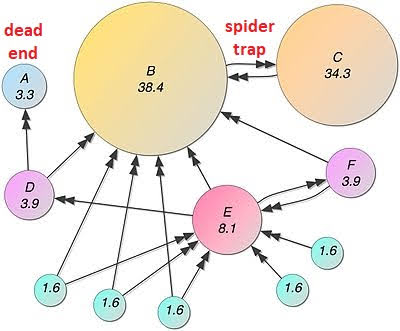
\includegraphics[width=0.60\textwidth]{out/about-pagerank.jpg}
  \caption{Example of web pages with hyperlinks and respective PageRanks \cite{pr-jardine07}.}
  \label{fig:about-pagerank}
\end{figure}

\vspace{2em}
\begin{algorithm}[!hbtp]
\caption{Algorithm for computing \emph{static PageRank} (static Monolithic). Here, $G$ is the current snapshot of the graph.}
\label{alg:pr-static}
\begin{algorithmic}
% \Require{$G$: Graph (V, E)}
\Function{staticPR}{$\vars{G}$}
\State $V \gets G.vertices$
\State $n \gets G.order$
\ForAll{$u \in V$} \textbf{in parallel}
  \State $prev_u = 1/n$
\EndFor
\Return{$\textsc{monolithicLoop}(G, [V], prev)$}
\EndFunction

\Statex

\Function{monolithicLoop}{$\vars{G}, \vars{SCCs}, \vars{prev}$}
  \State $MAX\_ITERS \gets 500$
  \State $\tau \gets TOLERANCE = 10^{-6}$
  \ForAll{$l \in range(0, MAX\_ITERS)$}
    \State $pr \gets \textsc{calculateRanks}(G, SCCs, prev)$
    \If{$l\infty{}Norm(prev, pr) < \tau$}
        \State $\textrm{break}$
    \EndIf
    \State $prev \gets pr$
  \EndFor
  \Return{$pr$}
\EndFunction

\Statex

\Function{calculateRanks}{$\vars{G}, \vars{SCCs}, \vars{prev}$}:
  \State $d \gets DAMPING = 0.15$
  \State $n \gets G.order$
  \State $outdeg \gets G.outDegrees$
  \ForAll{$SCC \in SCCs$} \textbf{in parallel}
    \ForAll{$v \in SCC$} \textbf{in parallel}
      \State $pr_v = d/n + (1 - d) * \Sigma _{u \in in(v)} \frac{prev_u}{outdeg_u}$
    \EndFor
  \EndFor
  \Return{$pr$}
\EndFunction
\end{algorithmic}
\end{algorithm}
\vspace{1em}


% Note that as originally conceived, the PageRank model does not factor a web browser's \textbf{back button} into a surfer's hyperlinking possibilities. Surfers in one class, if teleporting, may be much more likely to jump to pages about sports, while surfers in another class may be much more likely to jump to pages pertaining to news and current events. Such differing teleportation tendencies can be captured in two different \textbf{personalization vectors}. However, it makes the once query-independent, user independent PageRankings, user-dependent and more calculation-laden. Nevertheless, it seems this little personalization vector has had more significant side effects. This personalization vector, along with a \textbf{non-uniform/weighted} version of PageRank \cite{pr-dubey16} can help control spamming done by the so-called link farms \cite{pr-deeper01}.

PageRank algorithms almost always take the following \textbf{parameters}: damping, tolerance, and maximum number of iterations allowed. Here, \textbf{tolerance} defines the error between the previous and the current iterations. Though this is usually $L_1$-norm, $L_2$ and $L_\infty$-norm are also used sometimes. Both damping and tolerance control the rate of convergence of the algorithm. The choice of tolerance function also affects the rate of convergence. However, adjusting \textbf{damping} can give completely different PageRank values. Since the ordering of vertices is important, and not the exact values, it can usually be a good idea to choose a larger tolerance value.

Techniques to optimize the PageRank algorithm usually fall in two categories. One is to try \textbf{reducing the work per iteration}, and the other is to try \textbf{reducing the number of iterations}. Often, these goals are at odds against each other. The \textbf{adapting PageRank technique} "locks" vertices which have converged, and saves iteration time by skipping their computation \cite{pr-deeper01}. Identical nodes, which have the same in-links, can be removed to reduce duplicate computations and thus reduce iteration time. Road networks often have chains which can be short-circuited before PageRank computation to improve performance. Final ranks of chain nodes can be easily calculated. This reduces both the iteration time, and the number of iterations. If a graph has no dangling nodes, PageRank of each strongly connected component can be computed in topological order. This helps reduce the iteration time, number of iterations, and also enable concurrency in PageRank computation. The combination of all of the above methods is the \textbf{STIC-D algorithm} (see Figure \ref{fig:about-pagerank-sticd}) \cite{pr-sticd16}. A somewhat similar aggregation algorithm is \textbf{BlockRank} which computes the PageRank of hosts, local PageRank of pages within hosts independently, and aggregates them with weights for the final rank vector. The ranks of vertices for the entire graph can be found efficiently by computing the sub-PageRank of each connected component, and then using the sub-PageRanks together to form the global PageRank (Avrachenkov et. al. \cite{pr-avrachenkov04}). These methods exploit the inherent reducibility in the graph. The \textbf{Jacobi method} can also be used to compute the PageRank vector (Bianchini et. al. \cite{pr-bianchini05}) \cite{pr-deeper01}. \textbf{Monte Carlo} based PageRank methods consider several random walks on the input graph to get approximate PageRanks. Its optimizations for distributed PageRank computation (specially for undirected graphs) \cite{compute-frey13}, map-reduce algorithm for personalized PageRank \cite{pr-bahmani11}, and reordering strategy (to reduce space and compute complexity on GPU) for local PageRank \cite{pr-lai17} are present.

\begin{figure*}[hbtp]
  \centering
  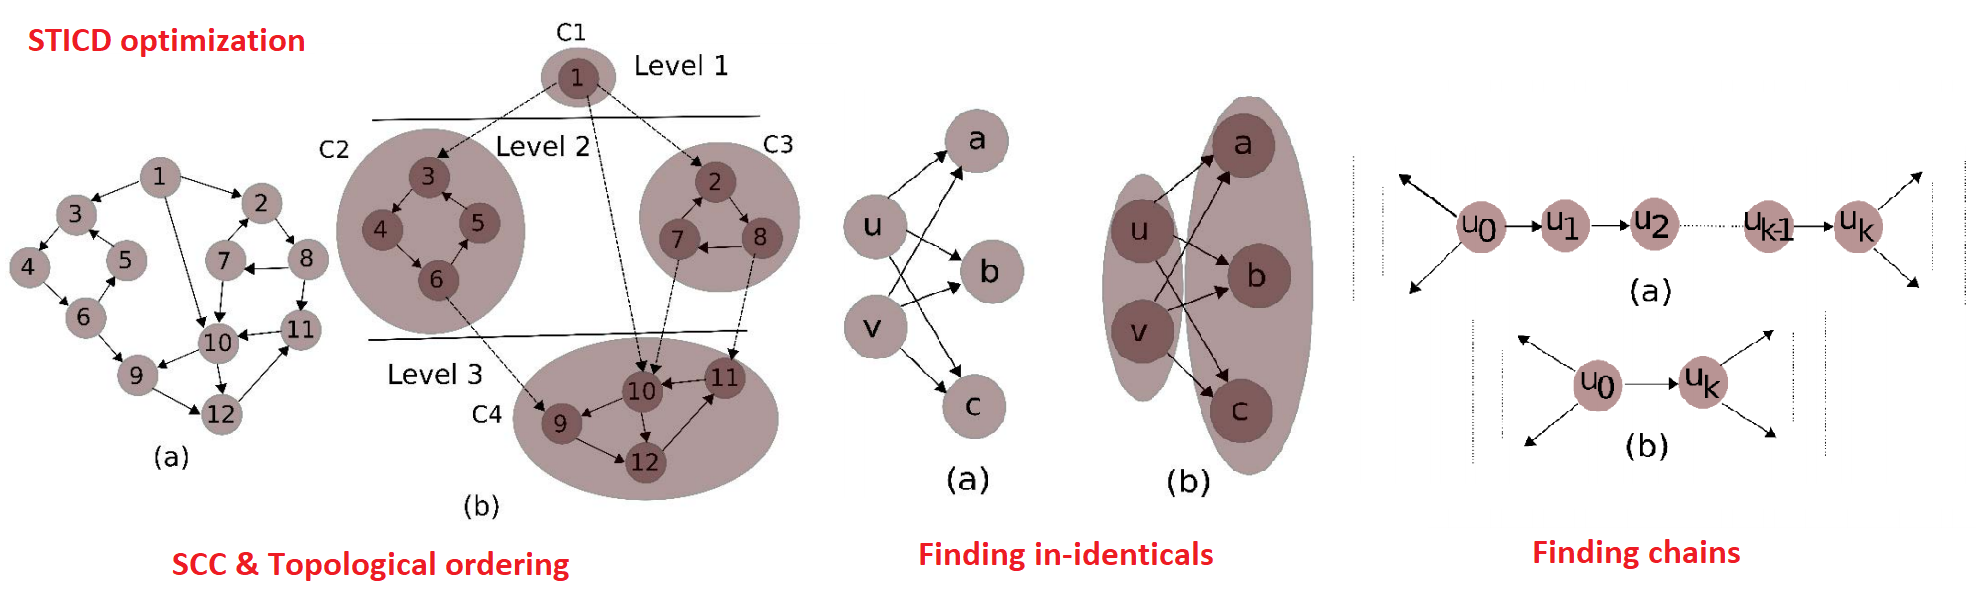
\includegraphics[width=0.98\textwidth]{out/about-pagerank-sticd.png}
  \caption{STIC-D: Algorithmic optimizations for PageRank \cite{pr-sticd16}.}
  \label{fig:about-pagerank-sticd}
\end{figure*}



% The time per iteration can be reduced further by taking note of the fact that the traditional algorithm is \textbf{not computationally bound} and \textbf{generates fine granularity random accesses} (it exhibits irregular parallelism). This causes poor memory bandwidth and compute utilization, and the extent of this is quite dependent upon the graph structure \cite{compute-hunold15} \cite{pr-lakhotia18}. \textit{Four strategies for neighbour iteration} were attempted, to help reason about the \textit{expected impact of a graph's structure} on the performance of each strategy \cite{compute-hunold15}. CPUs/GPUs are generally designed optimized to \textbf{load memory} in blocks (cache-lines in CPUs, coalesced memory reads in GPUs), and not for fine-grained accesses. Being able to adjust this behaviour depending upon application (PageRank) can lead to performance improvements. Techniques like \textit{prefetching to SRAM, using a high-performance shuffle network} \cite{graph-wang15}, \textit{indirect memory prefetcher (of the form $A[B[i]]$), partial cache line accessing mechanisms} \cite{memory-yu15}, \textit{adjusting data layout} \cite{pr-lakhotia18} \textit{(for sequential DRAM access} \cite{pr-zhou15} \textit{), and branch avoidance mechanisms (with partitioning)} \cite{pr-lakhotia18} are used. Large graphs can be \textbf{partitioned }or decomposed into subgraphs to help reduce cross-partition data access that helps both in distributed, as well as shared memory systems (by reducing random accesses). Techniques like \textit{chunk partitioning} \cite{pr-rungsawang12}, \textit{cache/propagation blocking} \cite{pr-beamer17}, \textit{partition-centric processing with gather-apply-scatter model} \cite{pr-lakhotia18}, \textit{edge-centric scatter-gather with non-overlapping vertex-set} \cite{pr-zhou17}, \textit{exploiting node-score sparsity} \cite{pr-li21}, and even \textit{personalized PageRank based partitioning} \cite{pr-mazaheri19} have been used. Graph/subgraph \textbf{compression} can also help reduce memory bottlenecks \cite{pr-rungsawang12} \cite{pr-guoqiang20}, and enable processing of larger graphs in memory. A number of techniques can be used to compress adjacency lists, such as, \textit{delta encoding of edge/neighbour ids} \cite{graph-bharat98}, and \textit{referring sets of edges in edge lists} \cite{graph-adler01} \cite{graph-raghavan03} (hard to find reference vertices though) \cite{pr-deeper01}. Since the rank vector (possibly even including certain additional page-importance estimates) must reside entirely in main memory, a few compression techniques have been attempted. These include \textit{lossy encoding schemes based on scalar quantization} seeking to minimize the distortion of search-result rankings \cite{pr-haveliwala02} \cite{pr-deeper01}, and using \textit{custom half-precision floating-point formats} \cite{pr-molahosseini20}.

As new software/hardware \textbf{platforms} appear on the horizon, researchers have been eager to test the performance of PageRank on the hardware. This is because each platform offers its own unique architecture and engineering choices, and also because PageRank often serves as a good benchmark for the capability of the platform to handle various other graph algorithms. Attempts have been made on distributed frameworks like \textit{Hadoop} \cite{pr-abdullah10}, and even \textit{RDBMS} \cite{compute-barolli21}. A number of implementations have been done on \textit{standard multicores} \cite{compute-barolli21}, \textit{Cell BE} \cite{compute-buehrer08} \cite{pr-zhou17}, \textit{AMD GPUs} \cite{pr-wu10}, \textit{NVIDIA/CUDA GPUs} \cite{pr-bisson16} \cite{pr-zhou17} \cite{graph-seo15}, \textit{GPU clusters} \cite{pr-rungsawang12}, \textit{FPGAs} \cite{pr-mughrabi21} \cite{graph-wang15} \cite{pr-guoqiang20}, \textit{CPU-FPGA hybrids} \cite{pr-hassan21} \cite{pr-usta21} \cite{pr-li21}, and even on SpMV \textit{ASICs} \cite{pr-sadi18}.

PageRank algorithm is a \textbf{live algorithm} which means that an ongoing computation can be paused during graph update, and simply be resumed afterwards (instead of restarting it). The first \textbf{updating} paper by Chien et al. \cite{pr-chien01} identifies a tiny region of the graph near the changed vertices/edges and model the remainder of the graph as a single vertex in a new, much smaller graph. PageRanks are computed for the small graph and then transferred to the original graph \cite{pr-deeper01}. A common technique used for dynamic PageRank algorithm, given a small change to the input graph, is to find the affected region in the preprocessing step with breadth-first search (BFS) or depth-first search (DFS) traversal from the vertices connecting the edges that were inserted or deleted \cite{pr-desikan05} \cite{pr-giri20}.




\section{Community Detection}

Communities are a groups of nodes in a network that correspond to functional units of a system (meta-nodes) \cite{com-chatterjee19}. \textbf{Community detection} schemes can be classified into three basic approaches: bottom-up, top-down, and data-structure based. The bottom-up approach includes the majority of algorithms, so further classification is possible \cite{com-souravlas21}. They can also be classified into three groups, namely: divisive, agglomerative, and multi-level (usually better) \cite{com-zarayeneh21}. The Louvain method for community detection extracts communities from large networks, and created by Blondel et al. \cite{com-blondel08} from the University of Louvain. It is a greedy optimization method with an average time complexity of $\Theta (n \log n)$, with $n$ being the total number of nodes in the network \cite{com-lancichinetti09}.

The idea behind this method is the optimization of modularity iteratively. \textbf{Modularity} is a metric that lies between -0.5 (non-modular communities) and 1 (fully modular communities) for any network, and measures the relative density of links inside communities in contrast to those outside communities. Optimizing modularity theoretically results in the best possible clustering of the nodes. However, as going through each possible clustering of the nodes is impractical, heuristic algorithms such a the Louvain method are used \cite{com-lancichinetti09}.

Louvain algorithm obtains hierarchical communities as a dendrogram through modularity optimization. Given an undirected weighted graph, all vertices are first considered to be their own communities. In the first phase, each vertex greedily decides to move to the community of one of its neighbors which gives the greatest increase in modularity. If moving to no neighbor's community leads to an increase in modularity, the vertex chooses to stay with its own community. This is done sequentially for all the vertices, as per the original algorithm. If the total change in modularity is more than a certain threshold, this phase is repeated. Once this \textbf{local moving phase} is complete, all vertices have formed their first hierarchy of communities. The next phase is called the \textbf{aggregation phase}, where all the vertices belonging to a community are collapsed into a single super-vertex, such that edges between communities are represented as edges between respective super-vertices (edge weights are combined), and edges within each community are represented as self-loops in respective super-vertices (again, edge weights are combined). Together, the local moving and the aggregation phases constitute a stage. This super-vertex graph is then used as input for the next stage. This process continues until the increase in modularity is below a certain threshold. As a result from each stage, we have a hierarchy of community memberships for each vertex as a dendrogram \cite{com-leskovec21}.

Approaches to perform the Louvain algorithm can be divided into \textbf{coarse-grained and fine-grained}. Coarse-grained approaches process a set of vertices in parallel, while fine-grained approaches process all vertices in parallel. A coarse-grained hybrid-GPU algorithm using multi GPUs has been implemented by Cheong et al. \cite{com-cheong13} which grabbed my attention. In addition, their algorithm does not use hashing for the local moving phase, but instead sorts each neighbor list based on the community id of each vertex \cite{com-naim17}.

It should be noted though that community detection methods such as the Louvain that rely on modularity maximization are known to suffer from \textbf{resolution limit problem}. This prevents identification of communities of certain sizes \cite{com-ghosh19}. The \textbf{other major community detection / clustering methods} include: Girvan-Newman or Edge betweenness, the Walktrap, the Louvain, and the CNM \cite{com-drakopoulos18}.

The Louvain algorithm has been implemented using \textbf{OpenMP} \cite{com-bhowmick13} \cite{com-lu15} \cite{com-sattar19}. Heuristics are used to break the sequential barrier \cite{com-lu15}, and load balancing is used to overcome the performance bottleneck \cite{com-sattar19}. It has also been implemented on \textbf{multicore platforms} \cite{com-fazlali17} \cite{com-gheibi20} \cite{part-hossain21} with adaptive parallel thread assignment \cite{com-fazlali17}, cache efficient implementation \cite{com-gheibi20}, and scatter instructions on 512-bit vectors (AVX-512) \cite{part-hossain21}. Platforms used range from an AMD multicore system \cite{com-fazlali17}, and Intel’s Knight's Landing, Haswell \cite{com-gheibi20}, SkylakeX, and Cascade Lake \cite{part-hossain21}. On \textbf{distributed systems} \cite{com-zeng18} \cite{com-ghosh19} \cite{com-sattar19}, the approaches use heuristics for coordinating community constitution in a distributed environment \cite{com-zeng18}, edge-balanced graph distribution for distributed memory implementation \cite{com-ghosh19}, and parallel load-balancing (OpenMPI) \cite{com-sattar19}. Platforms used range from Blue Gene/Q nodes \cite{com-zeng18}, P7-IH nodes \cite{com-zeng18}, and the ALCF Theta supercomputer \cite{com-ghosh19}.

Louvain algorithm based community detection has been implemented on single \cite{com-forster16} \cite{com-naim17} \cite{com-cheong13} \cite{com-mohammadi20} \cite{com-fontolan20} \cite{com-ghoshal19} \cite{com-sattar20} and multi-\textbf{GPUs} \cite{com-cheong13}. These methods use shared memory on the GPU, and use an optimal number of threads for computing modularity \cite{com-mohammadi20} \cite{com-naim17}. Sort-reduce paradigm with pruning on the input data \cite{com-fontolan20}, or hash-based approaches have been used \cite{com-naim17} \cite{com-fontolan20}. Hybrid CPU-GPU systems have been developed \cite{compute-hunold15} \cite{com-bhowmik19} \cite{com-souravlas20} \cite{com-alayyoub19} that use fine-grained parallelism on the GPU \cite{compute-hunold15}, and identify and move doubtful vertices between the devices \cite{com-bhowmik19}.
% Several parallelization heuristics for the Louvain algorithm have been implemented in Grappolo software library \cite{com-halappanavar17}. % Four major community detection algorithms have been implemented in Neo4j: Girvan-Newman or Edge betweenness, the Walktrap, the Louvain, and the CNM \cite{com-drakopoulos18}.

Some \textbf{improvements on the Louvain algorithm} include using a suitable heuristic based partitioning \cite{com-zeng15}, dealing with ghost vertices between graph partitions \cite{com-zeng15},  restricting the internal search rules \cite{com-ryu16}, and early pruning of the non-promising candidates \cite{com-ryu16}. Other interesting approaches include the use of MapReduce in a BigData batch processing framework \cite{com-zeitz17}. For cases where the dynamic graph can undergo abrupt changes, a change-aware model has been developed that detects the type of changes using least information \cite{com-samie17}.

% Community detection based on the \textbf{Infomap algorithm} \cite{com-zeng19} \cite{com-zeng18} \cite{com-faysal19} has been carried out by extending an existing asynchronous distributed framework while ensuring balanced workload and communication \cite{com-zeng19} \cite{com-faysal19}, and using a new heuristic to carefully coordinate the community constitution from the vertices to achieve convergence \cite{com-zeng18}. The Infomap algorithm finds communities by trying to minimize a cost function. The objsectionective is to try to minimize the cost of communicating across a random path between a sender and a receiver by trying to minimize the size of the message \cite{infomap-rosvall09} \cite{com-rita20}.

% Community detection has also been performed with the use of the \textbf{Label propagation algorithm}. It has pros with respect to its execution time, and the lack of additional information required about network structure. It however produces an aggregate of acceptable solutions, but not a unique one \cite{com-newman04}. At the start of the algorithm, each vertex is initialized with a unique label. These labels are then diffused across the graph. Well connected groups reach a common label quickly and continue to expand outwards until it is impossible to do so \cite{com-raghavan07}. A direction optimizing label propagation algorithm which utilizes frontiers, parameter controlled vertex processing order, and alternates between label push and pull operations, has been observed to reduce the number of edges visited and improve the quality of solution \cite{com-liu20}. GPU accelerated parallel label propagation implementation is also available that is able to deal with large-scale datasets that do not fit into GPU memory \cite{com-kozawa17}.

% Community detection based on the use of \textbf{genetic algorithm} \cite{com-taufan20} \cite{com-ghoshal19} \cite{com-lu20} has been achieved based on on diameter of the communities \cite{com-ghoshal19}, using multi-objective optimization with modularity index and a restricted diameter size of clusters \cite{com-lu20}, and adding a cleanup feature in process \cite{com-taufan20}.

% Other \textbf{alternative strategies to the Louvain algorithm} for community detection include combining multilevel graph contraction with core clustering algorithms \cite{com-ruan15}, using a divide and agglomerate algorithm \cite{com-liu19}, using the diameter of a community as a heuristic \cite{com-ghoshal17}, using the CEIL scoring function \cite{com-jain17}, using a game-theoretic approach based on modified modularity along with a new fitness function \cite{com-chopade17}, using fuzzy C-means and K-means algorithm \cite{com-alayyoub19}, using semi-supervised learning with Graph Convolutional Network (GCN) while applying mini-batch gradient descent for larger datasets \cite{com-sattar20}, and the Leiden algorithm which guarantees well connected communities through additional refinement steps in both the local-moving and agglomeration phase \cite{com-traag19}. Communities obtained with differing approaches can be compared with the following \textbf{metrics}: Modularity score \cite{com-ghoshal19}, Normalized Mutual Information (NMI) index \cite{com-jain17} \cite{com-chopade17}, and Jaccard Index \cite{com-jain17}.

% We now discuss a set of related papers in detail. The first paper is on “\textbf{Parallel Heuristics for Scalable Community Detection}” by Lu et al. \cite{com-lu15}. Here, the authors describe the issues with trying to parallelize: possibility of negative gain, community swapping, stuck in local optima. Heuristics like minimum labeling, vertex coloring, and vertex following. Implementation is in OpenMP C++ and they used STL map for communities each vertex is connected to (i was trying this with pre-counting instead which could be faster). They compare using modularity scores mostly. Specificity, Sensitivity, Overlap quality, and Rand index are difficult to calculate for large graphs (based on true positive, false positive, FN, TN). Modularity gain thresholds 10-2, 10-4. Comparison is also with label propagation based parallelization (PLM). There is also another community detection method called Clauset Newman Moore (CNM) which is agglomerative (cluster hierarchies tend to be more meaningful) \cite{com-lu15}.

% The second paper is on “\textbf{From Louvain to Leiden: guaranteeing well connected communities}” by Traag et al. \cite{com-traag19}. They show that some communities produced by the Louvain method are badly connected, and some even disconnected (and why this is not good). The Louvain method relies on modularity score, which has resolution issues (cant handle too small communities, solution CPM score). They add a refinement step and a better (random) local move approach. The restructuring phase is also with a refinement step. They also proved in the supplementary section why it's better \cite{com-traag19}.

% The third paper is on “\textbf{Community detection on the GPU}” by Naim et al. \cite{com-naim17}. The implementation in this paper uses the fine-grained approach such that each edge (not in all cases) is assigned a thread. Vertices are ordered by degree and partitioned by degree into buckets. For the smaller buckets, each edge is assigned a thread. For medium-degree buckets, multiple edges (in interleaved fashion) are assigned to each thread. For larger buckets, multiple vertices may be assigned to each thread block. Open addressing double-hashing is used for obtaining the total weight of communities linked to each vertex. For smaller buckets shared memory is used for storing the hash table, but for larger buckets, global memory is used. Due to global memory limits, execution of some large-degree vertices need to be performed sequentially. The size of a hash table is a precomputed prime number such that its size is at least 1.5 times the degree of the vertex. Note that community ids have to be stored as well. The algorithm implemented in this paper is lock free, and uses only atomic add and compare-and-swap (CAS) operations. Only moves of vertices from higher community id to lower community id are allowed to avoid race conditions. If two possible moves have the same delta-modularity, then the move to lower community id is chosen. Note that as the moving of vertices is performed in parallel, only community memberships of vertices from the previous iteration can be used (relaxed approach), unlike the sequential approach. Aggregation of communities into super-vertices in a new graph CSR is also performed on the GPU with similar thread management and hash tables \cite{com-naim17}. In addition, the authors employ the idea of using higher threshold for modularity gain in the initial rounds. Speedup is observed to be critically dependent upon threshold value. The relaxed strategy of local moving used here also leads to significantly reduced number of phases in certain cases, though this is offset by the algorithm spending more time in each iteration \cite{com-naim17}.

% The fourth paper is on “\textbf{Delta-Screening: A Fast and Efficient Technique to Update Communities in Dynamic Graphs}” by Zarayeneh et. al \cite{com-zarayeneh21}. In this paper, heuristics for skipping out most likely unaffected vertices for a modularity-based community detection method like Louvain and SLM (Smart Local Moving) is given. All edge batches are undirected, and sorted by source vertex id. For edge additions, source vertex i, highest modularity changing edge vertex j*, i's neighbors, and j*'s community are marked as affected. For edge deletions, where i and j must be in the same community, i, j, i's neighbors, and i's community are marked as affected. Performance is compared with static, dynamic baseline (incremental), and this method (both Louvain and SLM). Comparison is also done with "DynaMo" and "Batch" community detection methods \cite{com-zarayeneh21}.


\chapter{List of Selected Papers}
To carry out the research envisaged, the following papers are most relevant and provide important ideas / concepts / systems. We list out important contributions of each paper in detail.




\begin{longtable}[!hbtp]{|p{1cm}|p{11cm}|p{2cm}|}
% \centering
  \hline
  \textbf{S. No.} &
  \textbf{Paper} &
  \textbf{Citations} \\ \hline
  \endfirsthead
  \endhead
  \endfoot
  \endlastfoot

  1 &
  Prasanna Desikan, Nishith Pathak, Jaideep Srivastava, and Vipin Kumar. 2005. \textbf{Incremental page rank computation on evolving graphs}. In Special interest tracks and posters of the 14th international conference on World Wide Web (WWW '05). Association for Computing Machinery, New York, NY, USA, 1094–1095.\linebreak
  DOI: https://doi.org/10.1145/1062745.1062885 &
  54 \\ \hline
  \multicolumn{3}{|p{14cm}|}{This paper describes a simple method for computing dynamic pagerank, based on the fact that change of out-degree of a node does not affect its pagerank (first order markov property). The part of the graph which is updated (edge additions / edge deletions / weight changes) is used to find the affected partition of the graph using BFS. The unaffected partition is simply scaled, and pagerank computation is done only for the affected partition. \footnote{https://gist.github.com/wolfram77/f0a7534d49d5c07d4479ec3966c5d635}} \\ \hline

  2 &
  Yen-Yu Chen, Qingqing Gan, and Torsten Suel. 2002. \textbf{I/O-efficient techniques for computing pagerank}. In Proceedings of the eleventh international conference on Information and knowledge management (CIKM '02). Association for Computing Machinery, New York, NY, USA, 549–557.\linebreak
  DOI: https://doi.org/10.1145/584792.584882 &
  33 \\ \hline
  \multicolumn{3}{|p{14cm}|}{This paper describes a technique to partition the link file of the whole file into blocks of a range of destination nodes, with partial source nodes, so that it is possible to run power iteration of pagerank of massive graphs which do not fit in memory. The graphs must be stored on disk, and partitions of the graphs are scanned in every iteration until the ranks converge. Unlike Haveliwala's technique, this is similar to pull based pagerank. Both methods have similarities with join techniques in database systems. Topic-sensitive pagerank is also discussed which finds pagerank of graphs related to a specific keywords beforehand, and merges them together based upon the query (might return better results than global pagerank). This requires small adjustments to the random jump probability factor $(1-d)$. \footnote{https://gist.github.com/wolfram77/925cede0214aa0f391f34fa8ce137290}} \\ \hline

  3 &
  Paritosh Garg and Kishore Kothapalli. 2016. \textbf{STIC-D: algorithmic techniques for efficient parallel pagerank computation on real-world graphs}. In Proceedings of the 17th International Conference on Distributed Computing and Networking (ICDCN '16). Association for Computing Machinery, New York, NY, USA, Article 15, 1–10.\linebreak
  DOI: https://doi.org/10.1145/2833312.2833322 &
  7 \\ \hline
  \multicolumn{3}{|p{14cm}|}{In this paper, the authors exploit the reducibility of dead-end free graphs to compute PageRanks. They first split the vertices into strongly connected components (SCCs) and represent each SCC as a vertex in a block-graph. Each SCC is then processed as per its topological order in the block-graph. This enables them to reduce the operating memory requirement, thanks to the smaller size of SCCs that are processed in one go. As SCCs are processed in topological order, unnecessary iterations on vertices that are unlikely to converge are avoided. Processing vertices grouped into SCCs also improves performance due to inherent spatial locality within an SCC. In addition, this method allows SCCs residing on the same level in the block-graph to be processed independently of each other. This is demonstrated by the authors by processing each such SCC in parallel with OpenMP. They also present three algorithmic techniques for eliminating redundancies in PageRank computation, namely skipping repeated computation on in-identical vertices (minimize redundant computation), short circuiting chain vertices (help accelerate convergence), and skipping computation on vertices that appear to have converged (minimize redundant computation).The suitability of these techniques depend upon the nature of input graph. They study the techniques on four classes of real-world graphs: web graphs, social networks, citation and collaboration networks, and road networks. Their implementation achieves an average speedup of 32\% compared to a baseline implementation. \footnote{https://gist.github.com/wolfram77/bb09968cc0e592583c4b180243697d5a}} \\ \hline

  4 &
  Stergios Stergiou. 2020. \textbf{Scaling PageRank to 100 Billion Pages}. Proceedings of The Web Conference 2020. Association for Computing Machinery, New York, NY, USA, 2761–2767.\linebreak
  DOI: https://doi.org/10.1145/3366423.3380035 &
  1 \\ \hline
  \multicolumn{3}{|p{14cm}|}{In this paper, the author exploits the fact the communication required between iterations is identical. He uses this to develop a new communication format that allows significant reduction in bandwidth requirement. He experiments on massive web graphs with up to 38 billion vertices and 3.1 trillion edges, requiring a per-iteration time of 34.4 seconds, which is more than an order of magnitude improvement over the state-of-the-art. \footnote{https://gist.github.com/wolfram77/10964cd26f11f7a7299e7b74a0be7e7e}} \\ \hline

  5 &
  M. Naim, F. Manne, M. Halappanavar and A. Tumeo,  "\textbf{Community Detection on the GPU}," in 2017 IEEE International Parallel and Distributed Processing Symposium (IPDPS), Orlando, Florida, USA, 2017 pp. 625-634.\linebreak
  DOI: 10.1109/IPDPS.2017.16 &
  18 \\ \hline
  \multicolumn{3}{|p{14cm}|}{This paper discusses a GPU implementation of the Louvain community detection algorithm. The implementation in this report uses the fine-grained approach such that each edge (not in all cases) is assigned a thread. The algorithm implemented in this paper is lock free, and uses only atomic add and compare-and-swap (CAS) operations. Only moves of vertices from higher community id to lower community id are allowed to avoid race conditions. Aggregation of communities into super-vertices in a new graph CSR is also performed on the GPU with a similar thread management and hash tables. In addition, the authors employ the idea of using higher threshold for modularity gain in the initial rounds. Speedup is observed to be critically dependent upon threshold value. The relaxed strategy of local moving used here also leads to significantly reduced number of phases in certain cases, though this is offset by the algorithm spending more time in each iteration. \footnote{https://gist.github.com/wolfram77/7e72c9b8c18c18ab908ae76262099329}} \\ \hline

  6 &
  N. Zarayeneh and A. Kalyanaraman, "\textbf{Delta-Screening: A Fast and Efficient Technique to Update Communities in Dynamic Graphs}," in IEEE Transactions on Network Science and Engineering, vol. 8, no. 2, pp. 1614-1629, 1 April-June 2021.\linebreak
  DOI: 10.1109/TNSE.2021.3067665 &
  0 \\ \hline
  \multicolumn{3}{|p{14cm}|}{In this paper, heuristics for skipping out most likely unaffected vertices for a modularity-based community detection method like Louvain and SLM (Smart Local Moving) is given. All edge batches are undirected, and sorted by source vertex id. For edge additions, source vertex i, highest modularity changing edge vertex j*, i's neighbors, and j*'s community are marked as affected. For edge deletions, where i and j must be in the same community, i, j, i's neighbors, and i's community are marked as affected. Performance is compared with static, dynamic baseline (incremental), and this method (both Louvain and SLM). Comparison is also done with "DynaMo" and "Batch" community detection methods. \footnote{https://gist.github.com/wolfram77/c51f3580d7a76fa5c0a78491569df5ce}} \\ \hline

  7 &
  Brian Wheatman, Helen Xu. \textbf{A Parallel Packed Memory Array to Store Dynamic Graphs}. ALENEX 2021: Pages 31-45.\linebreak
  DOI: 10.1137/1.9781611976472.3 &
  3 \\ \hline
  \multicolumn{3}{|p{14cm}|}{Here they provide proof of a concurrently updateable data structure for dynamic graphs. It is an extension of CSR with free spaces in between so new edges can be added or removed. If there is no free space, edges can be redistributed within a tree-like hierarchy of blocks (leaves). If there is still no space, the size can be doubled. Looking up an edge still takes O(logN) like in CSR. They compare it to Aspen (dynamic graph streaming) and Ligra (static CSR) /Ligra+ (static compressed CSR) and find it to be close in performance to Ligra+ (Ligra slightly faster). Since PPCSR is not compressed and has free space, it occupies the most space. They use a (popcount based) lock order so that it is deadlock free. \footnote{https://gist.github.com/wolfram77/5e2e7349d062b9dfa1bbf0445c7c2e01}} \\ \hline

  8 &
  Qinggang Wang, Long Zheng, Yu Huang, Pengcheng Yao, Chuangyi Gui, Xiaofei Liao, Hai Jin, Wenbin Jiang, and Fubing Mao. 2021. \textbf{GraSU: A Fast Graph Update Library for FPGA-based Dynamic Graph Processing}. In The 2021 ACM/SIGDA International Symposium on Field-Programmable Gate Arrays (FPGA '21). Association for Computing Machinery, New York, NY, USA, 149–159.\linebreak
  DOI: https://doi.org/10.1145/3431920.3439288 &
  2 \\ \hline
  \multicolumn{3}{|p{14cm}|}{In this paper researchers focus on optimizing graph update though a caching technique using on-chip UltraRAM of FPGA. For dynamic graphs we can work on graph update, or graph algorithms. They work on graph updates. They list geomean speedup. For graph data structure they use Packed Memory Array (PMA) with CSR representation which supports fast edge addition and removal (I think they also mentioned use of fine-grained locking, instead of a per-vertex lock). A bitmap technique is used to avoid storing both UltraRAM and off-chip DRAM offsets. Algorithms to determine which vertex-edges to cache are run overlapped with graph algorithms (hidden overhead). It is based on "rich gets richer", that is high-degree vertices/recently updated vertices are most updated. Vertex data is stored in on-chip BRAM. Graph update is performed in batches. GraSU can be integrated with existing FPGA graph accelerators for static graphs. \footnote{https://gist.github.com/wolfram77/293b3a661759870482c7ceb21f1cb597}} \\ \hline

  9 &
  O. Green and D. A. Bader, "\textbf{cuSTINGER: Supporting dynamic graph algorithms for GPUs}," 2016 IEEE High Performance Extreme Computing Conference (HPEC), 2016, pp. 1-6.\linebreak
  DOI: 10.1109/HPEC.2016.7761622 &
  24 \\ \hline
  \multicolumn{3}{|p{14cm}|}{These people wrote the first data structure for maintaining dynamic graphs with NVIDIA CUDA GPUs. Unlike STINGER which uses a block linked-list and GT-STINGER which uses Array of Structures (AoS), here they instead used Structure of Arrays (SoA) which is not only more suitable to GPU memory access, but also allows smaller allocations modes (memory is a premium in GPU). They use a custom memory manager which speeds up memory management (instead of using system memory manager). The data structure used is the standard adjacency list (CSR) and pointers are updated when the edge list has to grow. It could handle upto 10 million updates per second (large batch sizes), and ran a static graph algorithm (triangle counting) 1-10\% slower. This shows that cuSTINGER can also be used with static graph algorithms. Dynamic graph algorithms should run much faster. \footnote{https://gist.github.com/wolfram77/a4e430a45be95abad16c52643261a966}} \\ \hline

  10 &
  M. Besta, M. Fischer, V. Kalavri, M. Kapralov and T. Hoefler, "\textbf{Practice of Streaming Processing of Dynamic Graphs: Concepts, Models, and Systems}" in IEEE Transactions on Parallel \& Distributed Systems (2021), vol. no. 01, pp. 1-1, 5555.\linebreak
  DOI: 10.1109/TPDS.2021.3131677 &
  10 \\ \hline
  \multicolumn{3}{|p{14cm}|}{This is a huge review paper discussing a lot about several graph streaming frameworks, and graph databases. GPU frameworks given are cuSTINGER, EvoGraph, Hornet, faimGraph, GPMA. Gap between databases and frameworks seems to be closing. \footnote{https://gist.github.com/wolfram77/7e2a17af8ec541ddcaf3344ec9b90edf}} \\ \hline

% \vspace{0.3 cm}
\caption{List of Selected papers}
\label{tab:papers}
\end{longtable}


\chapter{Parallel Dynamic Algorithms for Computing PageRank}
From chapter 2, we observe that a number of techniques have been studied for optimizing the performance of the PageRank algorithm. This is important, since one of the most important applications of PageRank, that is the ordering of search results on the web for a given query, requires operating on massive-scale graphs. Considering the fact that these graphs are constantly being updated, a number of techniques for dynamic PageRank computation have been developed. To date, powerful shared memory systems have achieved the best performance. This is thanks to the availability of multicore servers with more than a terabyte of memory, which can fit graphs with hundreds of billions of edges. These shared-memory multicores are significantly more efficient on time and energy basis, when compared to when compared to distributed memory systems \cite{graph-shun13}. In order to cope with low memory systems, streaming PageRank techniques have been developed which do not require storing the entire graph in memory for the computation \cite{pr-sarma11}.

% However, we find that most studies focus only on the teleport-based dead end handling strategy for PageRank, as recommended by the Original Google patent. Thus, algorithmic optimization techniques that could be applied to other dead end handling strategies were left behind. Through our experimentation, we observe that teleport-based PageRank has the lowest performance among three other strategies.
The paper on STIC-D based algorithmic techniques for PageRank \cite{pr-sticd16} utilizes the decomposability of graphs. It allows for greater parallelization, given its lack of per-iteration communication requirement. It also serves as a good foundation for exact streaming PageRank since only a subset of the needs to be processed at a time. Given the demand for PageRank computation across disciplines, a study focused on the design of GPU-based implementation of the algorithm is essential.

% We also noted issues with performance comparison between the technique developed, and the state of the art in a few papers. This was because of the difference in choice of error measurement function, and measurement of time taken for computation, among other things. Average speedup in some cases was obtained by finding the speedup of the developed technique for each test case, and averaging them. The standard approach in the domain of bench-marking involves the use of geometric mean (GM). Thus, we find a detailed study of the effects of variations on the performance of PageRank to be essential before the development of a new optimization technique. This would help us pin down the factors that allow a certain technique to perform better than others.

Our initial focus is on collecting data on the effects of adjusting PageRank parameters, error measurement functions, and dead end handling strategies, and rank adjustment strategies. We develop a CUDA-based PageRank to act as a baseline for future PageRank techniques on the GPU.
The design of STIC-D based algorithmic techniques for PageRank \cite{pr-sticd16} involves both monolithic (non-decomposed) and levelwise (decomposed) versions. This helps with determining the factors that contribute to performance improvement. We expect that this analysis would in turn help with development of any further techniques or optimizations. Since some optimization techniques only work for a specific category of graphs, we wish to automatically determine the choice of using an optimization. Further study involves applying the developed techniques to streaming PageRank on the GPU.

% Individual repositories for each specific experiment would be maintained. This is in order to enable easy peer-review, as well as enabling other people easily verify the results for themselves. Additional helper packages would be written as per requirement. Integrations with existing graph frameworks may be done, if time permits.
% We have studied the effects of adjusting various aspects of the PageRank algorithm, and developed two suitable approaches for dynamic PageRank computation on the CPU, as well as the GPU. We hope this would be a stepping stone for us in developing suitable dynamic and streaming algorithms for massive real-world graphs.




% \section{PageRank Algorithm}

We first attempt to parallelize PageRank for the NVIDIA Volta GPU. The first step of our parallelization process is to independently parallelize map and reduce-like operations within the algorithm, to obtain a suitable implementation and launch config. The second step involves parallelizing the rank computation process using a \emph{switched thread/block-per-vertex} approach after the vertices have been partitioned by in-degree at a suitable switch point, and with apt launch configs for each partition. We observe that the sequential CPU-based vector element sum with 32-bit floating point values suffers from precision issues, while the CUDA-based does not.
% We first attempt to parallelize PageRank for the NVIDIA Volta GPU. GPUs are usually optimized for \emph{chunked memory access patterns} and \emph{high compute}. While the PageRank algorithm has an \emph{unchunked-gather memory access pattern} and \emph{low compute}, implementing it on a CUDA-enabled GPU, such as the Volta GV100, can bring a significant performance improvement. The first step of our parallelization process is to independently parallelize map and reduce-like operations within the algorithm, to obtain a suitable implementation and launch config. The second step involves parallelizing the rank computation process using a \emph{switched thread/block-per-vertex} approach after the vertices have been partitioned by in-degree at a suitable switch point, and with apt launch configs for each partition.
% Compared to nvGraph PageRank on fixed and temporal graphs, we observe a small performance improvement. We should however note that the CUDA implementation we develop here uses L1-norm for error measurement, while nvGraph PageRank uses L2-norm for error measurement, along with a per iteration L2-norm rank scaling followed by an L1-norm rank scaling after the final iteration. We should also remark that the sequential CPU-based vector element sum with 32-bit floating point values suffers from precision issues, while the CUDA-based does not.

% \begin{figure*}[!hbtp]
  \centering

  \subfloat{
    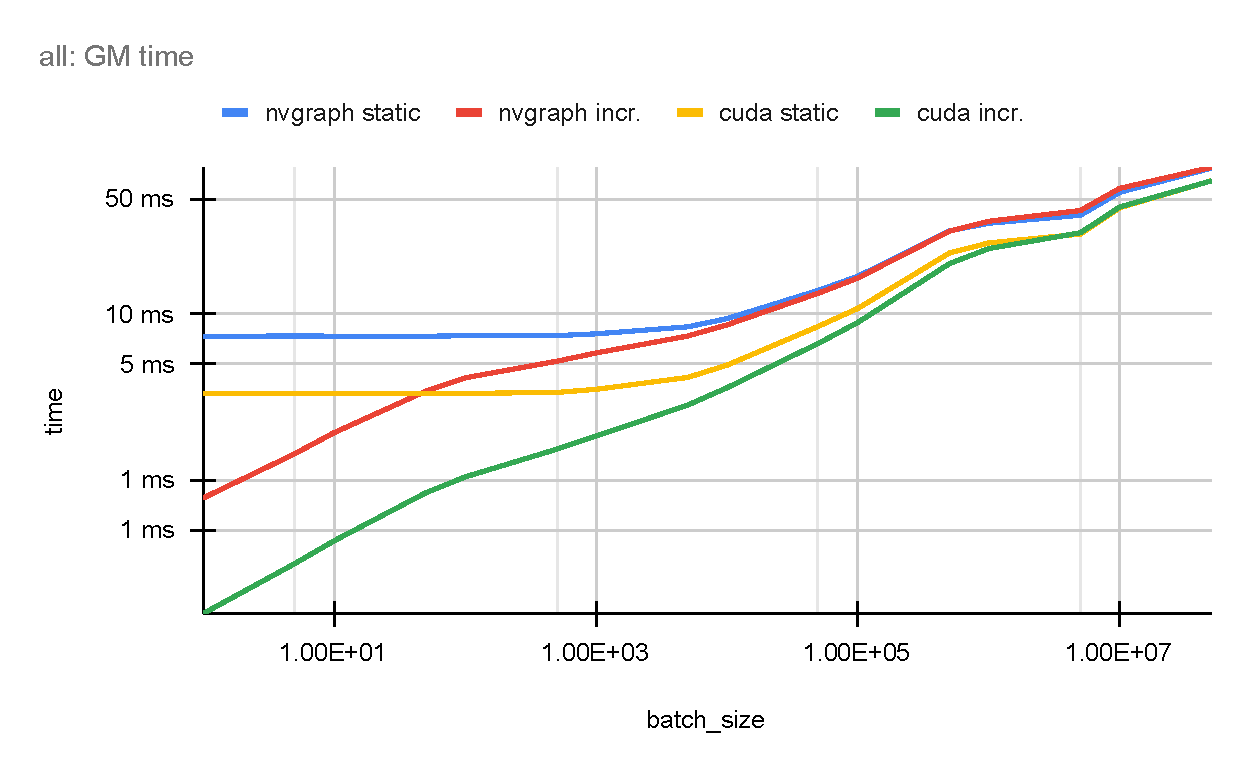
\includegraphics[width=0.48\textwidth]{out/pr-cuda-st-vs-it-time.pdf}
    \label{fig:pr-cuda-st-vs-it-time}
  }
  \subfloat{
    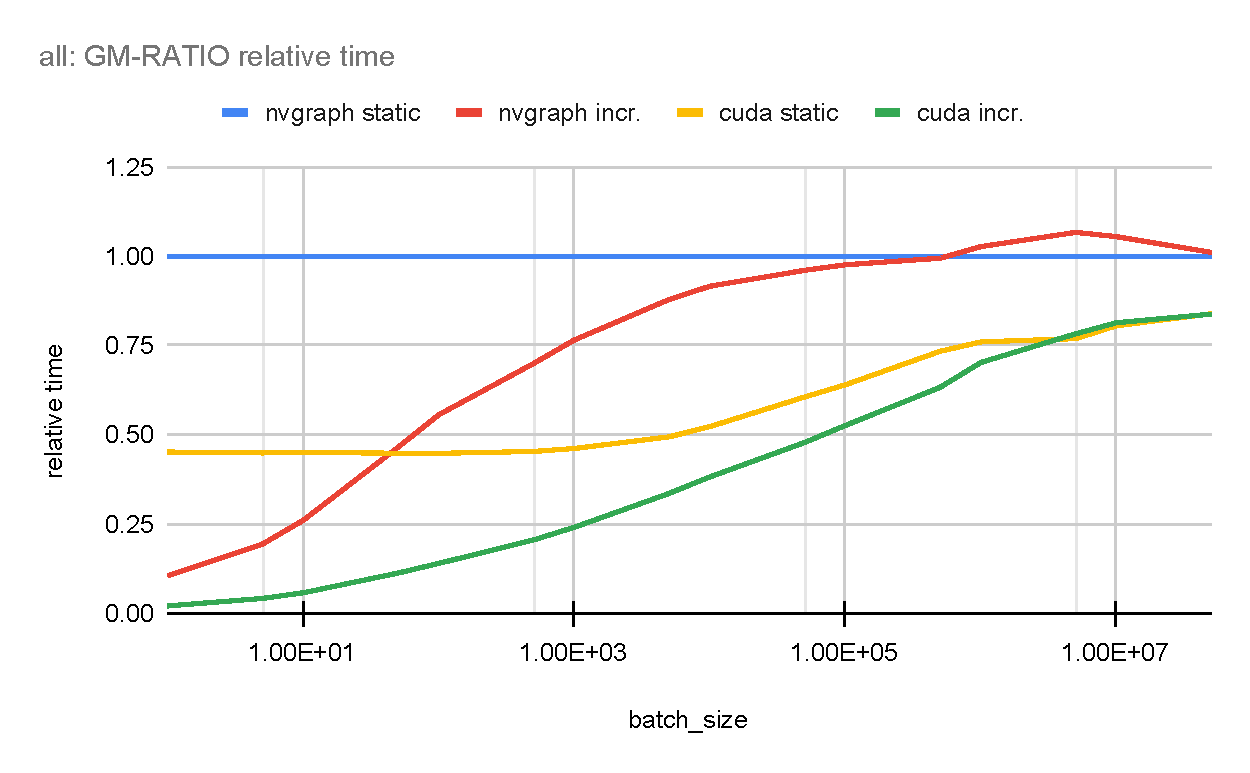
\includegraphics[width=0.48\textwidth]{out/pr-cuda-st-vs-it-rtime.pdf}
    \label{fig:pr-cuda-st-vs-it-rtime}
  }

  \caption{GM time taken for static and incremental PageRank with nvGraph and CUDA implementation, with respect to nvGraph’s static PageRank is shown on the left. Relative GM time taken is shown on the right. This is done on seven temporal graphs. Error measurement between the previous and current iteration is done using L1-norm except for nvGraph, which uses L2-norm instead. Batch sizes range from $10^0$ to $5 * 10^7$.}
  \label{fig:pr-cuda-st-vs-it}
\end{figure*}



We then look into the effect on PageRank computation time for different datatypes of the rank vector and the CSR representation of graphs on both a CPU as well as a GPU. Results indicate that using a wider datatype for the CSR representation has a smaller impact to performance compared to using a wider datatype for the rank vector. This can be explained from the fact that the PageRank algorithm accesses the CSR representation in a linear-like fashion, which improves the cache hit ratio for a CPU, and improves memory coalescing for a GPU. On the other hand, it accesses the rank vector in random order. When a wider datatype is used, a higher memory bandwidth is required, and if memory accesses are random, cache memory can get occupied faster and require faster evictions, slowing down performance. In all cases however, the impact on performance for a wider datatype is higher for GPU, compared to CPU. This is likely because of architectural differences between the two devices, with the GPU having a wider memory bus than the CPU.
% We then look into the effect on PageRank computation time for different datatypes of the rank vector and the CSR representation of graphs. We try this on both a CPU, as well as a GPU. Results indicate that using a wider datatype for the CSR representation has a smaller impact to performance compared to using a wider datatype for the rank vector. This is despite the fact that the CSR representation has a much larger memory footprint, and thus higher memory access requirement, than the rank vector. This can be explained from the fact that the PageRank algorithm accesses the CSR representation in a linear-like fashion, which improves the cache hit ratio for a CPU, and improves memory coalescing for a GPU.
% On the other hand, it accesses the rank vector in random order. When a wider datatype is used, a higher memory bandwidth is required, and if memory accesses are random, cache memory can get occupied faster and require faster evictions, slowing down performance. In all cases however, the impact on performance for a wider datatype is higher for GPU, compared to CPU. This is likely because of architectural differences between the two devices, with the GPU having a wider memory bus than the CPU.

% \begin{figure*}[!hbtp]
  \centering

  \subfloat{
    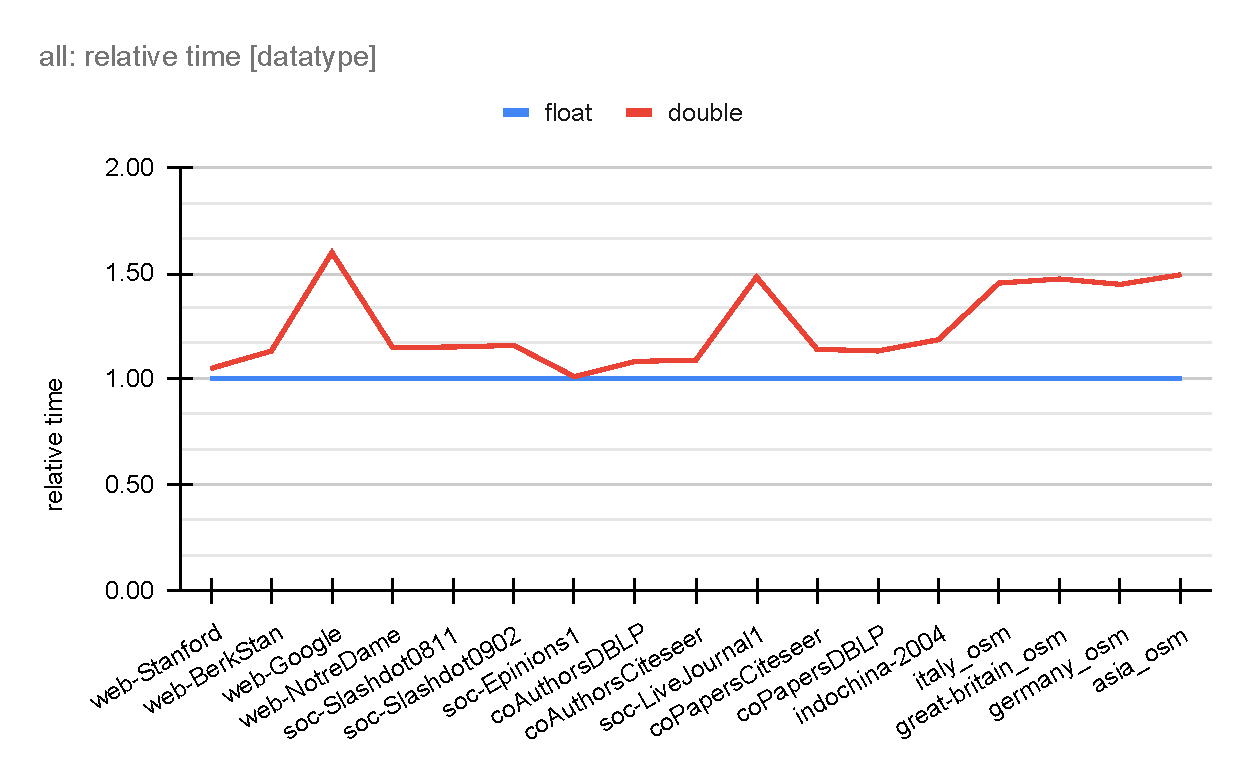
\includegraphics[width=0.48\textwidth]{out/pr-cuda-adj-rtype-rtime.pdf}
    \label{fig:pr-cuda-adj-rtype-rtime}
  }
  \subfloat{
    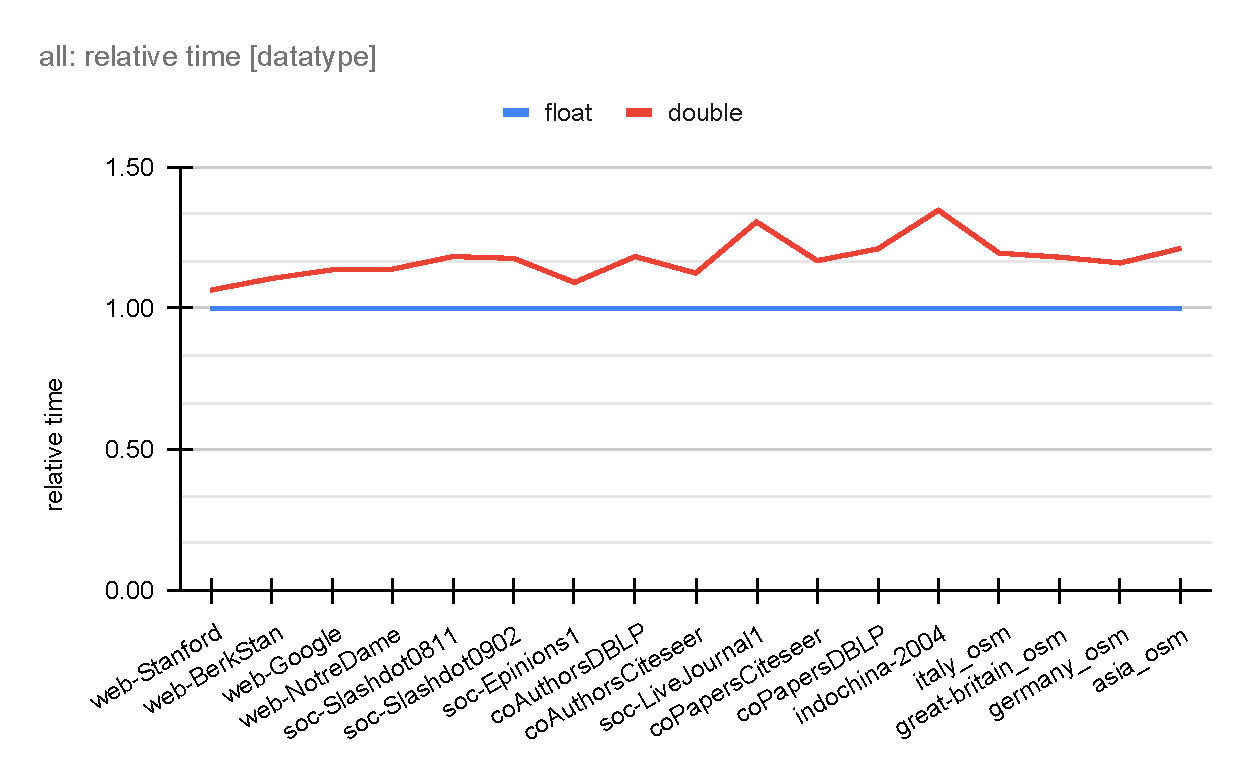
\includegraphics[width=0.48\textwidth]{out/pr-cuda-adj-ctype-rtime.pdf}
    \label{fig:pr-cuda-adj-ctype-rtime}
  }

  \caption{Relative time taken for switched thread/block-per-vertex CUDA-based (GPU) PageRank computation with the following datatypes for the rank vector is shown on the left: 32-bit floating point (float), 64-bit floating point (double). Relative time taken for CSR representation with the following datatypes is shown on the right: 32-bit integer (int32), 64-bit integer (int64). This is done on 5 web graphs, 4 social networks, 4 collaboration networks, and 4 road networks.}
  \label{fig:pr-cuda-adj-type}
\end{figure*}



We then explore the performance benefits of five different algorithmic optimizations for PageRank as presented in STIC-D paper \cite{pr-sticd16}, but without splitting the computation of ranks into multiple levels. The first two include splitting vertices by components, and sorting components by topological order in block-graph. The remaining three optimizations include skipping computation on in-identical, chain, and converged vertices. Again, we do this on both a CPU, as well as a GPU.
Our results indicate that splitting vertices by components provides a small performance improvement on average on both the devices. However, sorting components provides little additional benefit. The other three optimizations are beneficial only on certain graphs, but are detrimental on others due to their associated cost. Therefore, skip in-identical and chain optimizations should be applied only on graphs with a large number of in-identical and chain vertices respectively. In contrast, as the applicability of skip converged optimization cannot be predicted beforehand, it can be ignored. Moreover, in all cases the impact on performance is lower for GPU, compared to CPU. This is possibly because of the warp divergence introduced by the three skip optimizations due to irregular skipping of rank computation of vertices.

% \begin{figure*}[!hbtp]
  \centering

  \subfloat{
    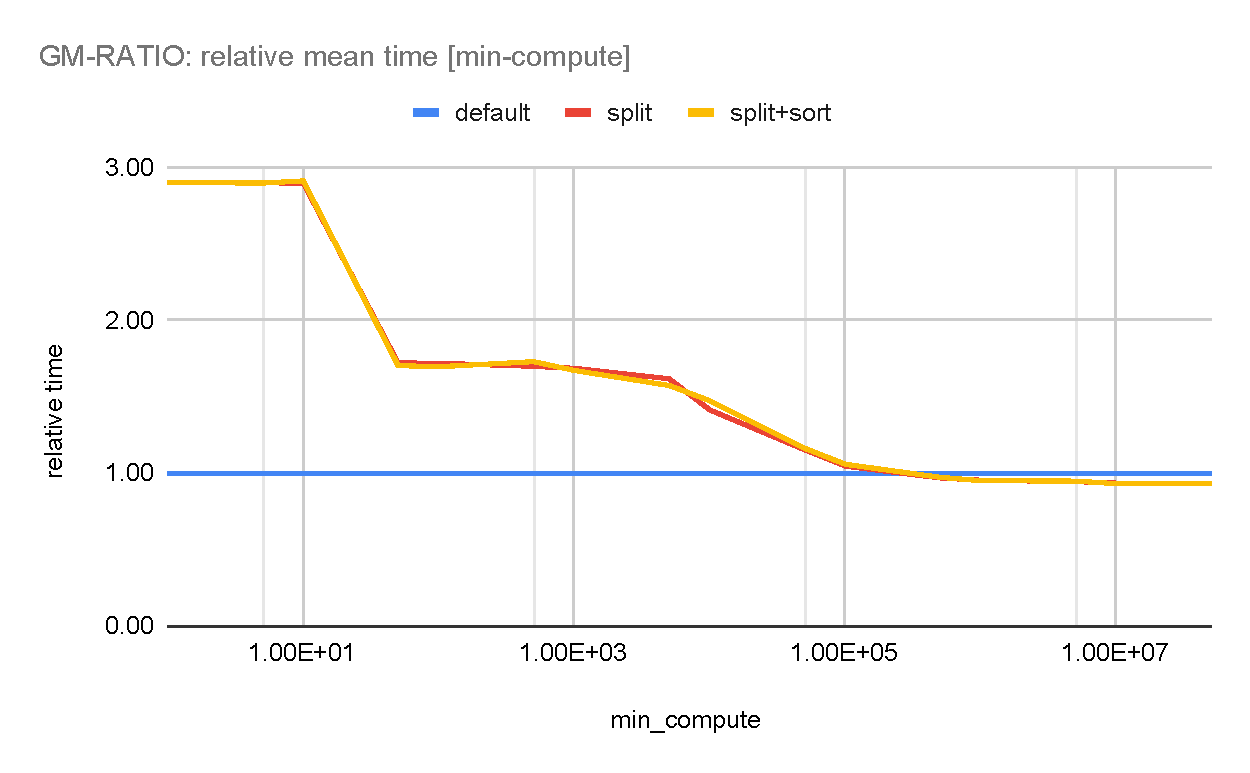
\includegraphics[width=0.48\textwidth]{out/pr-cuda-opt-s-rtime.pdf}
    \label{fig:pr-cuda-opt-s-rtime}
  }
  \subfloat{
    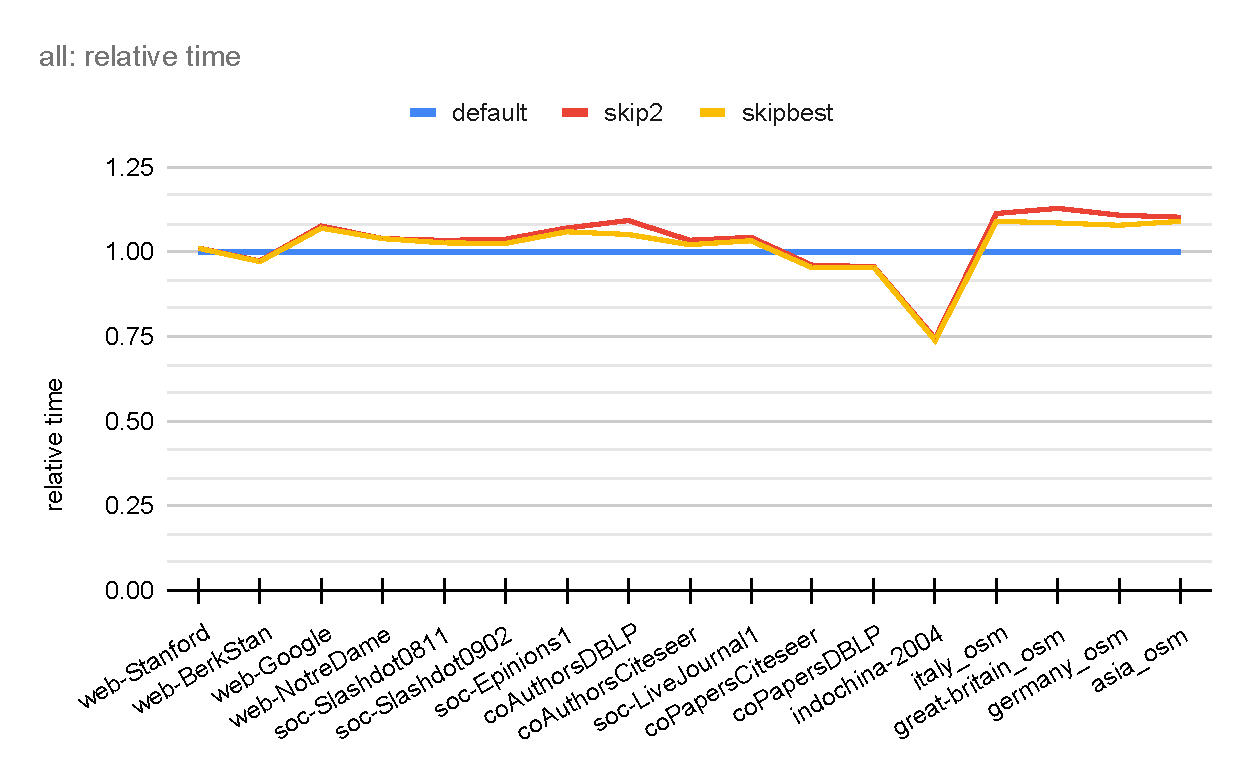
\includegraphics[width=0.48\textwidth]{out/pr-cuda-opt-i-rtime.pdf}
    \label{fig:pr-cuda-opt-i-rtime}
  }

  \caption{\textbf{Left:} Relative GM of time taken on all graphs for switched thread/block-per-vertex CUDA-based (GPU) static PageRank computation with the following algorithmic optimizations: no optimization (default), split vertices by components (split), and split vertices by components with each component sorted in topological order of its block-graph  (split+sort). This is relative to no optimization, with min. compute size ranging from 1 to 5×107. \textbf{Right:} Rel. time taken for switched thread/block-per-vertex CUDA-based (GPU) static PageRank computation with the following algorithmic optimizations: no optimization (default), skip all in-identicals (skip2), and skip in-identicals of best min. size  (skipbest). The ratio is obtained with respect to no optimization. This is done on 5 web graphs, 4 social networks, 4 collaboration networks, and 4 road networks.}
  \label{fig:pr-cuda-opt-si}
\end{figure*}

% \begin{figure*}[!hbtp]
  \centering

  \subfloat{
    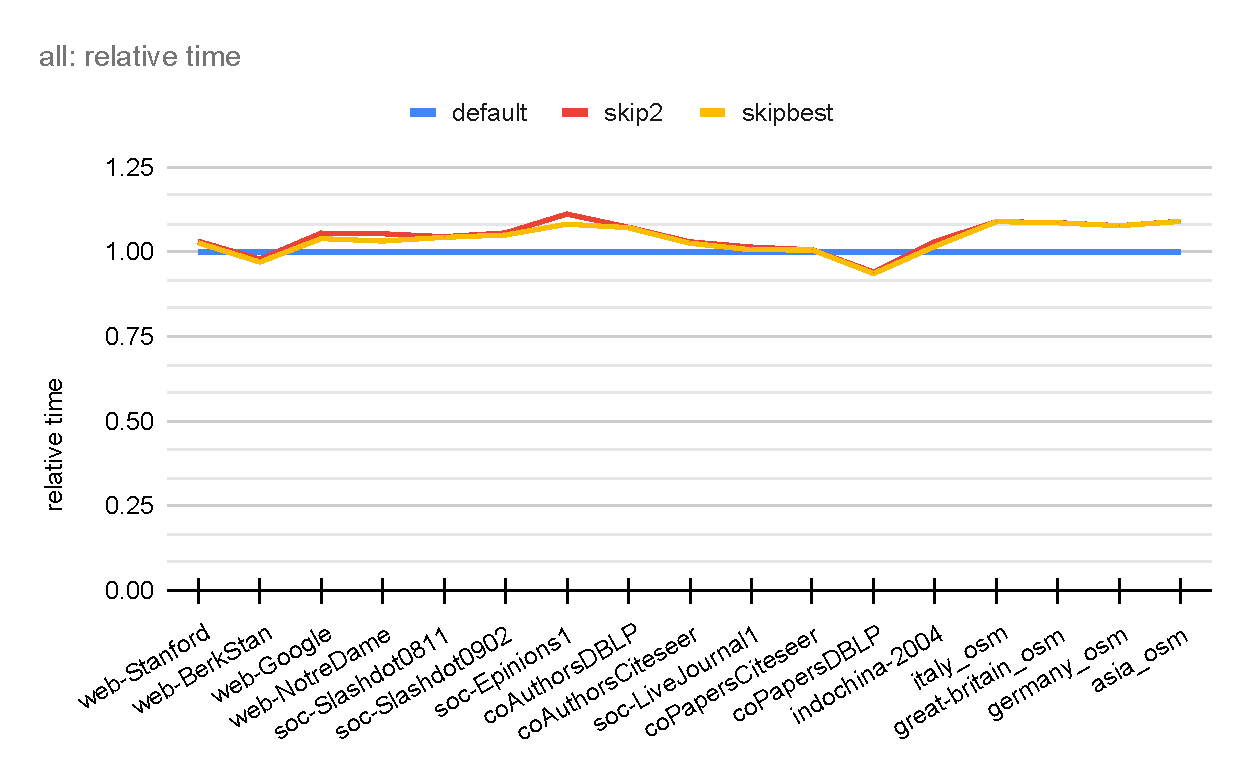
\includegraphics[width=0.48\textwidth]{out/pr-cuda-opt-c-rtime.pdf}
    \label{fig:pr-cuda-opt-c-rtime}
  }
  \subfloat{
    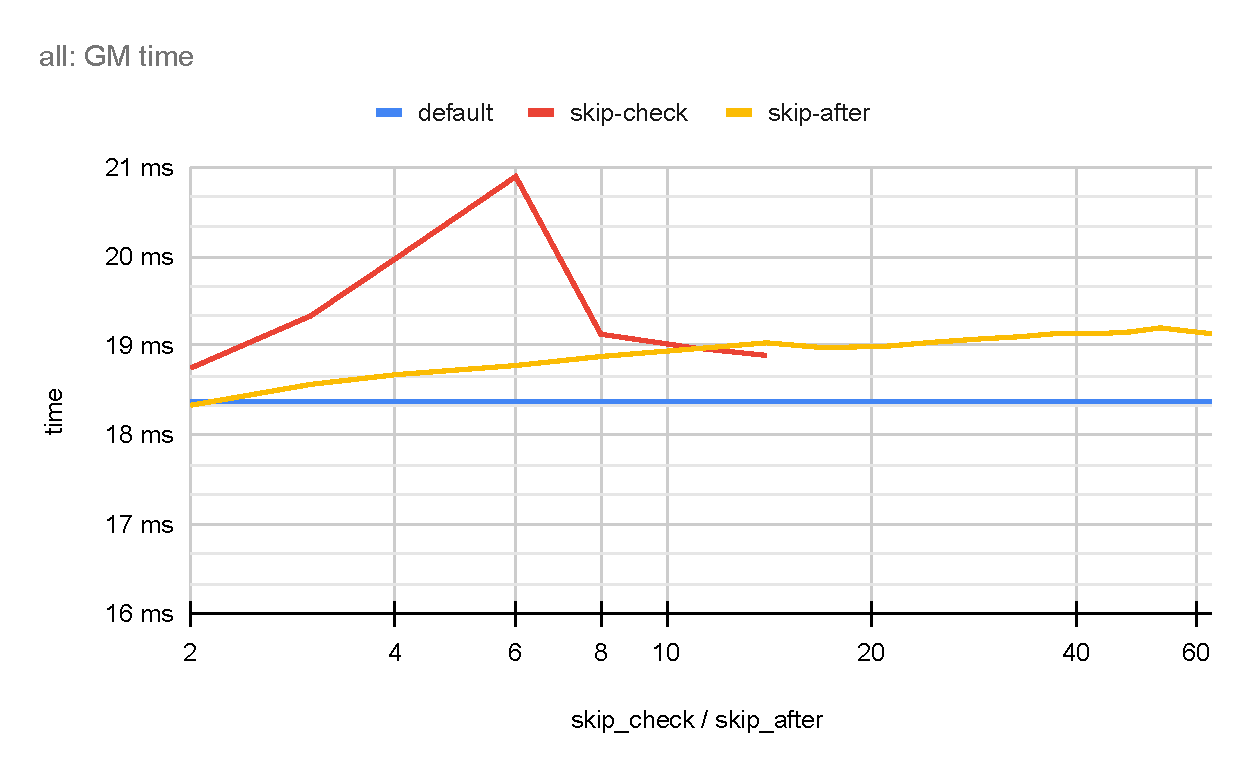
\includegraphics[width=0.48\textwidth]{out/pr-cuda-opt-d-time-gm.pdf}
    \label{fig:pr-cuda-opt-d-time-gm}
  }

  \caption{\textbf{Left:} Relative time taken for switched thread/block-per-vertex CUDA-based (GPU) static PageRank computation with the following algorithmic optimizations: no optimization (default), skip all chains (skip2), and skip chains of best min. size  (skipbest). The ratio is obtained with respect to no optimization. \textbf{Right:} GM of time taken on all graphs for switched thread/block-per-vertex CUDA-based (GPU) static PageRank computation with the following algorithmic optimizations: no optimization (none), skip converged vertices with recheck every X turns (skip-check), and skip converged vertices after X turns  (skip-after). This is relative to no optimization, with skip-check ranging from 2 to 16, and skip-check ranging from 2 to 64 (separately). Each of this is done on 5 web graphs, 4 social networks, 4 collaboration networks, and 4 road networks.}
  \label{fig:pr-cuda-opt-cd}
\end{figure*}



We then present two parallel algorithms for updating the PageRank values of vertices in a dynamic graph. Our techniques require the recomputation of the PageRank of only the vertices affected by the insertion/deletion of a batch of edges. One algorithm named \levelwisePR{}, as shown in Algorithm \ref{alg:pr-levelwise}, computes updated ranks of vertices in topological order of affected SCCs, avoiding unnecessary recomputation of SCCs that are dependent upon ranks of vertices in other SCCs which have not yet converged. We start by recomputing the PageRanks of vertices in the SCCs grouped by levels in the block-graph of the updated graph. PageRank computation is then performed on each affected level in sequential order from the topmost unprocessed level until convergence. This is repeated until all affected SCCs have been processed. The other algorithm named \monolithicPR{}, as shown in Algorithm \ref{alg:pr-monolithic}, computes updated ranks of vertices in one go, but groups vertices by SCCs and partitions them by in-degree, to obtain a better work-balance on the GPU. We first identify all the affected SCCs of updated graph. PageRank computation is then performed on all affected SCCs in every iteration, until all affected vertices appear to have converged (based on given tolerance).

\vspace{2em}
\begin{algorithm}[!hbtp]
\caption{Algorithm for computing \emph{dynamic Levelwise PageRank}. Here, $F$ is the previous snapshot of the temporal graph, $G$ is the current snapshot, and $prev$ is the initial estimate of pr (usually it is the \emph{adjusted} previous pr of vertices).}
\label{alg:pr-levelwise}
\begin{algorithmic}
\Function{dynamicLevelwisePR}{$\vars{F}, \vars{G}, \vars{prev}$}
  \State $SWITCH\_DEG \gets 64$ \Comment{indegree}
  \State $SCCs \gets affectedSCCs(F, G)$
  \State $mergeByLevel(SCCs, G)$
  \If{$GPU$}
    \State $partitionByIndeg(SCCs, G, SWITCH\_DEG)$
  \EndIf
  \Return{$\textsc{levelwiseLoop}(G, SCCs, prev)$}
\EndFunction

\Statex

\Function{levelwiseLoop}{$\vars{G}, \vars{SCCs}, \vars{prev}$}
  \State $pr \gets prev$
  \ForAll{$SCC \in SCCs$}
    \State $pr \gets \textsc{monolithicLoop}(G, [SCC], pr)$ \\  \Comment{see Algorithm \ref{alg:pr-static}}
  \EndFor
  \Return{$pr$}
\EndFunction
\end{algorithmic}
\end{algorithm}
\vspace{1em}
\vspace{2em}
\begin{algorithm}[!hbtp]
\caption{Algorithm for computing \emph{dynamic Monolithic PageRank}. Here, $F$ is the previous snapshot of the temporal graph, $G$ is the current snapshot, and $prev$ is the initial estimate of ranks (usually it is the \emph{adjusted} previous ranks of vertices).}
\label{alg:pr-monolithic}
\begin{algorithmic}
\Function{dynamicMonolithicPR}{$\vars{F}, \vars{G}, \vars{prev}$}
  \State $MIN\_WORK \gets 10^7$ \Comment{vertices}
  \State $SWITCH\_DEG \gets 64$ \Comment{indegree}
  \State $SCCs \gets affectedSCCs(F, G)$
  \If{$GPU$}
    \State $mergeMiniSCCs(SCCs, G, MIN\_WORK)$
    \State $partitionByIndeg(SCCs, G, SWITCH\_DEG)$
  \EndIf
  \Return $\textsc{monolithicLoop}(G, SCCs, prev)$ \\  \Comment{see Algorithm \ref{alg:pr-static}}
\EndFunction
\end{algorithmic}
\end{algorithm}
\vspace{1em}


Both algorithms accept the previous and current snapshot of a graph as input, along with the current (initial) ranks of the vertices. SCCs of both graph snapshots are obtained using Kosaraju's algorithm and compared, in order to obtain a list of changed SCCs. From each SCC, depth-first search (DFS) is performed in order to obtain a list of affected SCCs. We use the Compressed Sparse Row (CSR) representation of graphs for PageRank computation in order to have good memory locality. Vertices are reordered as part of preprocessing step, and computed ranks are un-reordered as part of post-processing step.

We achieve good device utilization and load balance across threads in our GPU implementation as follows. As the degree of vertices may be varying widely, we follow the general practice of choosing a thread or block of threads per vertex for calculating ranks. In order to achieve this, vertices in each SCC with an in-degree $64$ (see $SWITCH\_DEG$ in Algorithm \ref{alg:pr-monolithic}) or below are considered to be the thread-per-vertex partition where a CUDA kernel assigns the work of calculating the rank for each vertex to a single thread (belonging to a block of $512$ threads). For vertices with in-degree greater than  $64$, a CUDA kernel assigns the work of calculating the ranks of each such vertex to a block of threads (consisting of $256$ threads). We observe that grouping vertices by SCCs, and processing each SCC with a thread-per-vertex and a block-per-vertex CUDA kernel after partitioning yields better performance. Hence, this is the approach taken here. However, small affected SCCs are combined together until they satisfy a minimum work requirement of 10 million vertices (see $MIN\_WORK$ in Algorithm \ref{alg:pr-monolithic}). We do this in order to reduce the number of kernel calls. Further details of the implementation is given in our code repository \footnote{Code for this work, https://github.com/puzzlef/pagerank-multi-monolithic-vs-levelwise}.

We first compare the performance of \monolithicPR{} and \levelwisePR{} with state-of-the-art approaches. In particular, we compare our multicore implementations with the plain STIC-D algorithm (static Levelwise) \cite{pr-sticd16}, which is a static algorithm in the sense that they perform a full recomputation on the new graph. We compare our GPU implementations with the naive dynamic version of nvGraph library implementation of PageRank on a GPU \cite{pr-nvgraph}, a simplified dynamic algorithm which does not skip processing of unaffected vertices (nvGraph does not provide any parameter to control the number of vertices to be processed). We experiment with batch sizes of 500, 1000, 2000, 5000, and 10000 edges. The results of this experiment on both the CPU and the GPU is shown in Figure \ref{fig:pr-mono-vs-levl-time}. As can be noted from these figures, on the CPU, \monolithicPR{} and \levelwisePR{} achieve an average speedup of 6.1\x and 8.6\x respectively, over the STIC-D algorithm. On the GPU, \monolithicPR{} and \levelwisePR{} achieve an average speedup of 9.8\x and 9.3\x respectively, over the PageRank algorithm from the nvGraph library. We observe that \levelwisePR{} performs better on the CPU compared to \monolithicPR{}. \levelwisePR{} is computationally more efficient because it processes SCCs in topological order, avoiding unnecessary recomputation of SCCs that are dependent upon ranks of vertices in other SCCs which have not yet converged. We also observe that \monolithicPR{}{} performs better on the GPU compared to \levelwisePR{}. This is likely due to the presence of levels with insufficient work to keep the GPU busy.

We also compare the performance of our algorithms with HyPR \cite{pr-giri20}, a state-of-the-art dynamic PageRank algorithm that only recomputes ranks of affected vertices in the graph. The algorithm from HyPR runs in heterogeneous mode and utilizes both the CPU and the GPU simultaneously. To keep our comparison fair, we modify the source code of HyPR to exclusively run either on a CPU or a GPU. We run all the algorithms with a similar set of batches as above. As seen in Figure \ref{fig:pr-mono-vs-levl-time}, we observe a mean speedup of {4.2\x} and {5.8\x} for algorithms \monolithicPR{} and \levelwisePR{} respectively on the CPU, over a pure CPU implementation of HyPR. On the GPU, we observe a mean speedup of {1.9\x} and {1.8\x} for \monolithicPR{} and \levelwisePR{} respectively, over a pure GPU implementation of HyPR. The speedups can be attributed to grouping of vertices by SCCs and partitioning by in-degree in case of \monolithicPR{}, and due to the processing of affected SCCs in topological ordering in case of \levelwisePR{}.

We then contrast the performance of a batched update to a series of single edge updates (cumulative). We observe that a batch update of 5000 edges offer a speedup of 4066\x and 2998\x respectively for the monolithic and levelwise approaches on the CPU, and a speedup of 1712\x and 2324\x respectively on the GPU, as shown in Figure \ref{fig:pr-mono-vs-levl-batch}.

We observe that \levelwisePR{} is a suitable approach for CPUs. However on a GPU, smaller levels/components could be combined and processed at a time in order to help improve GPU usage efficiency as \monolithicPR suggests.
On graphs with a single SCC, the performance of the levelwise approach is noted to be almost indistinguishable from the monolithic approach. This is because a single SCC implies a single level in the block-graph for Levelwise approach to process, making its behavior is identical to that of monolithic.

\begin{figure*}[!hbtp]
  \centering

  \subfloat{
    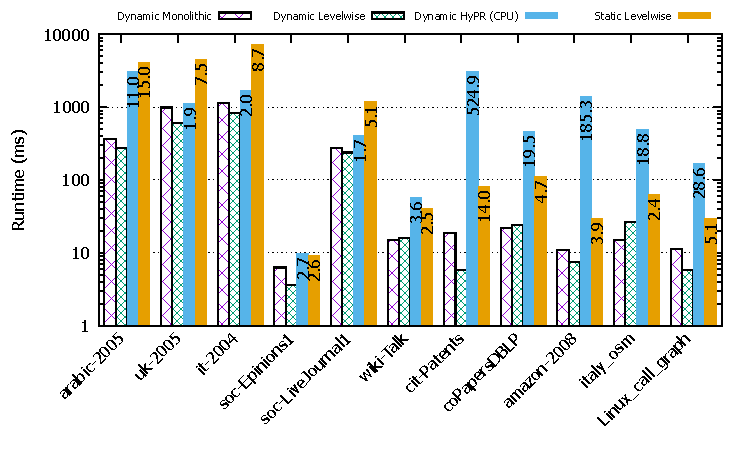
\includegraphics[width=0.48\textwidth]{out/pr-mono-vs-levl-omp-time.pdf}
    \label{fig:pr-mono-vs-levl-omp-time}
  }
  \subfloat{
    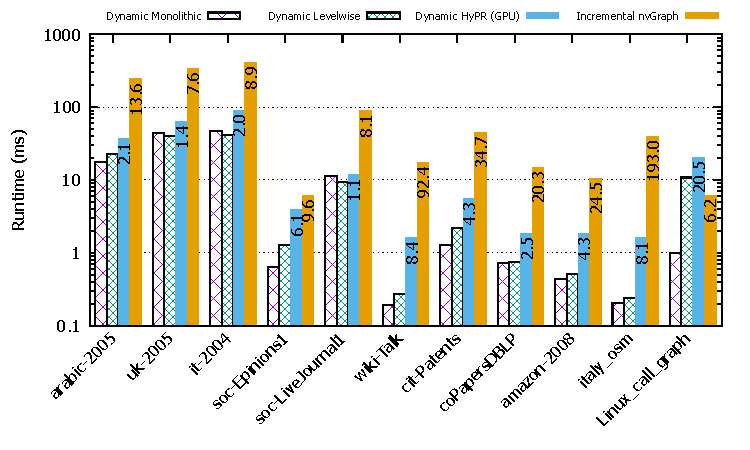
\includegraphics[width=0.48\textwidth]{out/pr-mono-vs-levl-cuda-time.pdf}
    \label{fig:pr-mono-vs-levl-cuda-time}
  }

  \caption{Time taken for PageRank computation with  \monolithicPR{} and \levelwisePR{} for various batch sizes on the CPU (shown on the left) and the GPU (shown on the right). Batch sizes of 500, 1000, 2000, 5000, and 10000 are used. Time taken with \emph{pure CPU implementation of HyPR} and \emph{plain STIC-D PageRank (static Levelwise)} on the CPU, and speedup of \levelwisePR{} over the two approaches (labeled on top of the respective bars) is also included for comparison. Time taken with \emph{pure GPU implementation of HyPR} and \emph{incremental nvGraph PageRank} on the GPU, and speedup of \monolithicPR{} over the two approaches is included as well.}
  \label{fig:pr-mono-vs-levl-time}
\end{figure*}

\begin{figure*}[!hbtp]
  \centering

  \subfloat{
    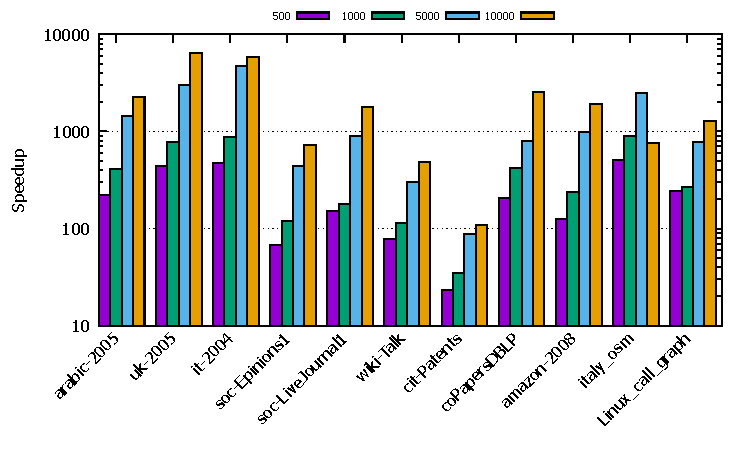
\includegraphics[width=0.48\textwidth]{out/pr-levl-omp-batch.pdf}
    \label{fig:pr-levl-omp-batch}
  }
  \subfloat{
    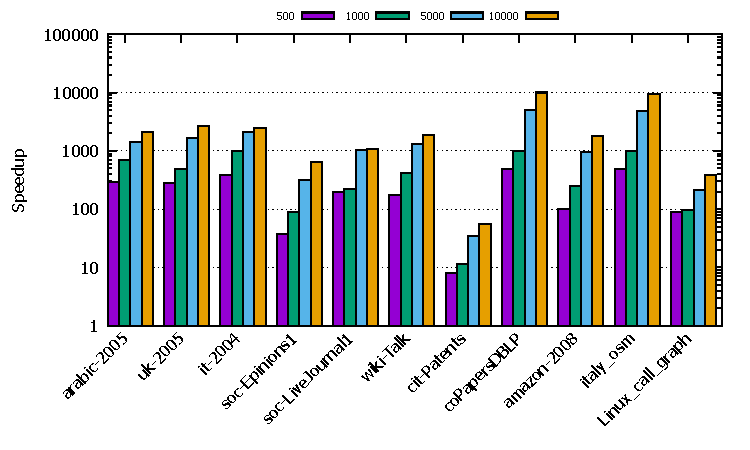
\includegraphics[width=0.48\textwidth]{out/pr-mono-cuda-batch.pdf}
    \label{fig:pr-mono-cuda-batch}
  }

  \caption{Speedup of batched \levelwisePR{} algorithm with respect to cumulative single-edge updates with the same approach on the CPU is shown on the left. Speedup of batched \monolithicPR{} algorithm with respect to cumulative single-edge updates with the same approach on the GPU is shown on the right. Batch sizes of 500, 1000, 5000, and 10000 are shown.}
  \label{fig:pr-mono-vs-levl-batch}
\end{figure*}





% We then extend the levelwise strategy of PageRank computation in the STIC-D paper to perform dynamic PageRank on the CPU as well as the GPU. We compare it to our previous monolithic CPU/GPU implementations, along with other state-of-the art implementations, such as nvGraph and HyPR. We experiment with batch sizes of 500, 1000, 2000, 5000, and 10000 edges.
% On the CPU, the monolithic and levelwise approaches achieve an average speedup of 6.1\x and 8.6\x respectively, over the STIC-D algorithm \cite{pr-sticd16}. On the GPU, an average speedup of 9.8\x and 9.3\x respectively is achieved over the PageRank algorithm from the nvGraph library. We observe a mean speedup of 4.2\x and 5.8\x respectively on the CPU, over a pure CPU implementation of HyPR \cite{hipc19}. On the GPU, we observe a mean speedup of 1.9\x and 1.8\x respectively, over a pure GPU implementation of HyPR, as shown in figure \ref{fig:pr-mono-vs-levl-time}.


\chapter{Further Studies planned}
\section{PageRank Algorithm}

We consider massive graphs that do not fit on a single machine. To process the PageRank values of the graph as streams of updates arrive, we would need a distributed collection of machines, such as a multi-GPU or a multi-CPU collection. We think of a primary/secondary model where the primary receives the updates and works along with the secondaries to process the update as a sliding-window.

The secondaries store pieces of the graph as a partitioning of the graph. The primary has to keep track of which vertex is in which partition and hence in which secondary. This information should be stored in light-weight data structure at the primary since the space at the primary is not to exceed $O(|V|)$. So, the partitioning structure should also help keep the size of this information small. Our approach for this could include the use of multiple bloom filters instead of using a large hash-table.

% \singlespacing
Beyond the storage, the solution has the following main steps:
\begin{itemize}[itemsep=-1.5em,topsep=0em]
% \topsep -1em
% \itemsep -1.5em
\item Receive a batch of updates at the primary.
\item Use the data structure at the primary to identify the secondaries that own the edges in the update.
\item Send the edges to the respective secondaries.
\item Process the edges at each secondary in a parallel manner.
\item Any global computation as needed across the secondaries.
\item Update the partition structure as needed.
\end{itemize}
% \onehalfspacing

Answers to the above questions depend on the nature of partitioning used. If the partitioning is based on strongly connected components, then, the storage at the primary can be $O(n)$. We will keep vertex id, component id, and secondary id for each vertex. Based on the computation also, there may be additional communication needed between the secondaries. In the case of PageRank, we will also have some dependencies in terms of which components need the final PageRank values from other components.




\section{Community Detection}

Community detection is a memory intensive operation, similar to PageRank. We note that dynamic community detection based on the Louvain algorithm using a delta-screening approach has been proposed that prunes out nodes that are unlikely to change communities on a given graph delta. This has been implemented with a sequential algorithm on the CPU \cite{com-zarayeneh21}. We intend to adapt this approach onto the GPU, which would enable users of the algorithm with a significantly reduced computation time. For this, we would use a GPU implementation of the static Louvain algorithm as our baseline \cite{com-naim17}.

We plan to use the Compressed Sparse Row (CSR) format for representing the graph on the GPU. This also includes aggregate super-vertex graphs, which would be created through device code based on the results of the local moving phase. For vertex-to-community determination in the local moving phase, we wish to explore the impact of hash vs sort based approaches.

It should be noted that both the PageRank and the Louvain algorithm (especially) require a significant number of indirect memory accesses. This can be somewhat managed by the GPU through automatic warp switching. However, this is not an ideal solution as it introduces additional latency and has increased power consumption. Similar to how processor in memory (PIM) architectures are being explored in the field of machine learning, we wager that indirect memory access architectures, such as the IMP \cite{memory-yu15}, would be a part of memory hardware used for graph processing. It may be noted that paging in memory is already a form of indirect memory access, though it is handled by the CPU, not the DRAM. We therefore would like to explore the possible performance improvement achievable with such hardware through detailed simulations.


\appendix
\small
\bibliographystyle{IEEEtran}
\bibliography{inc/References}
\end{document}
